   % Arrest rate pretrends

   \begin{figure}[h]
    \centering
    \caption{Adult Black Arrest Rate Per 100,000}%
    \subfloat[\centering 1986]{{\includegraphics[width=7cm]{pretrends/1986/ab.png} }}%
    \qquad
    \subfloat[\centering 2010]{{\includegraphics[width=7cm]{pretrends/2010/ab.png} }}%
    \label{fig:raw_ab}%
  \end{figure}
  \begin{figure}[h]
    \centering
    \caption{Juvenile Black Arrest Rate Per 100,000}%
    \subfloat[\centering 1986]{{\includegraphics[width=7cm]{pretrends/1986/ab.png} }}%
    \qquad
    \subfloat[\centering 2010]{{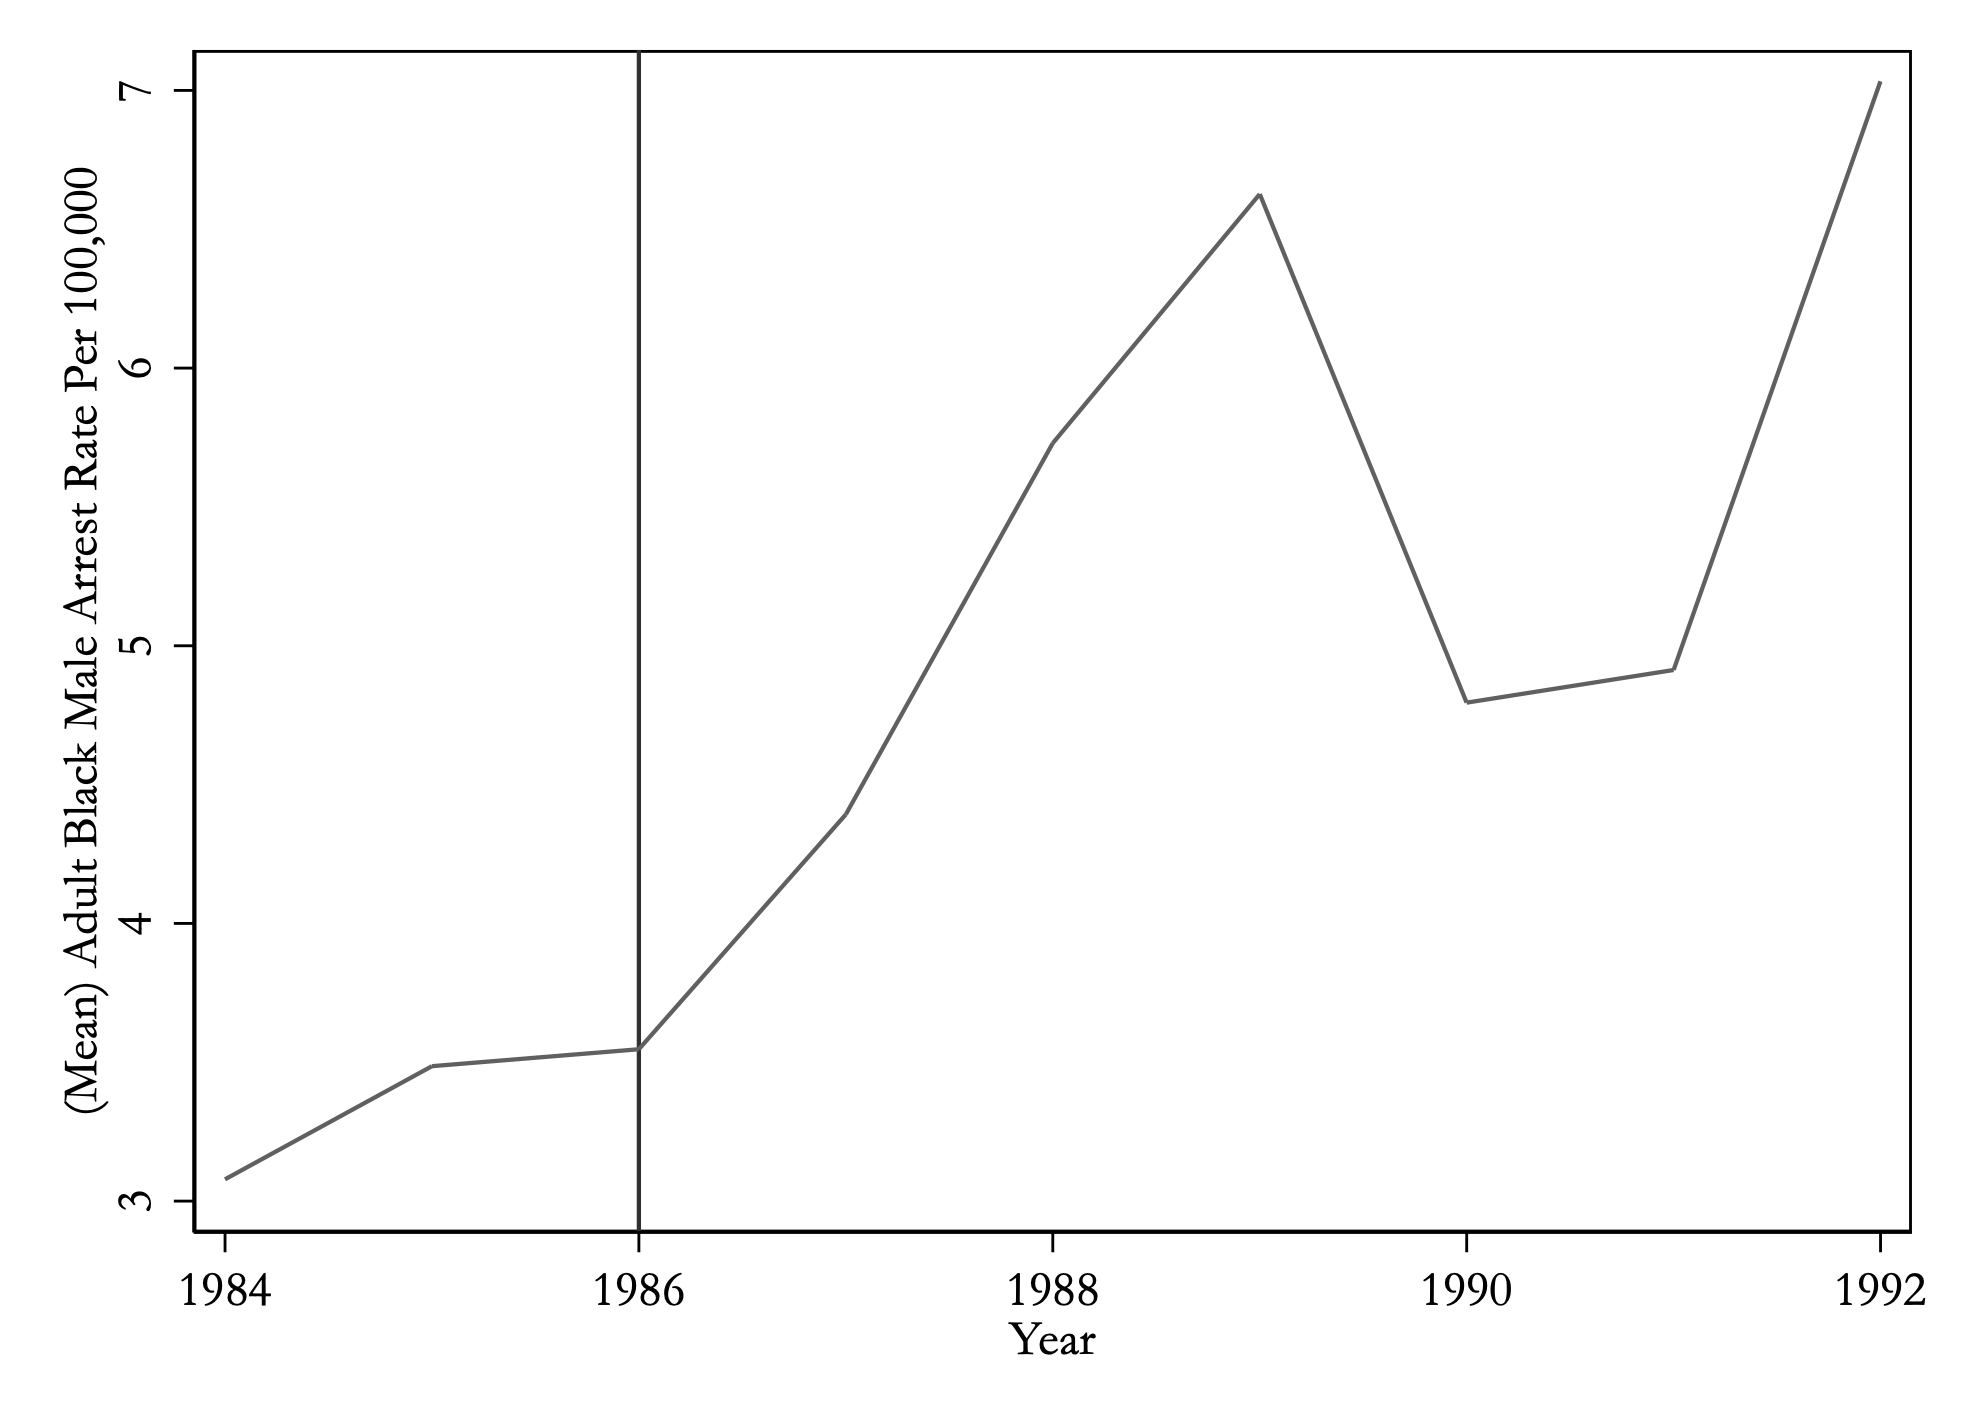
\includegraphics[width=7cm]{pretrends/2010/jb.png} }}%
    \label{fig:raw_jb}%
  \end{figure}

  \begin{footnotesize}
    \noindent Note: These figures report the drug crime arrest rate per 100,000 for black adults and black juveniles separately over time using CPS-UCR merged data from 1984-1992 and 2005-2016. A vertical line is drawn to denote the passage of the Anti-Drug Abuse Act of 1986 and the Fair Sentencing Act of 2010.
  \end{footnotesize}
  
  \clearpage
  
  % High vs low arrest states pretrends

  \begin{figure}[h]
    \centering
    \caption{College Enrollment By States with High vs Low Black Adult Drug Arrest Rates}%
    \subfloat[\centering 1986]{{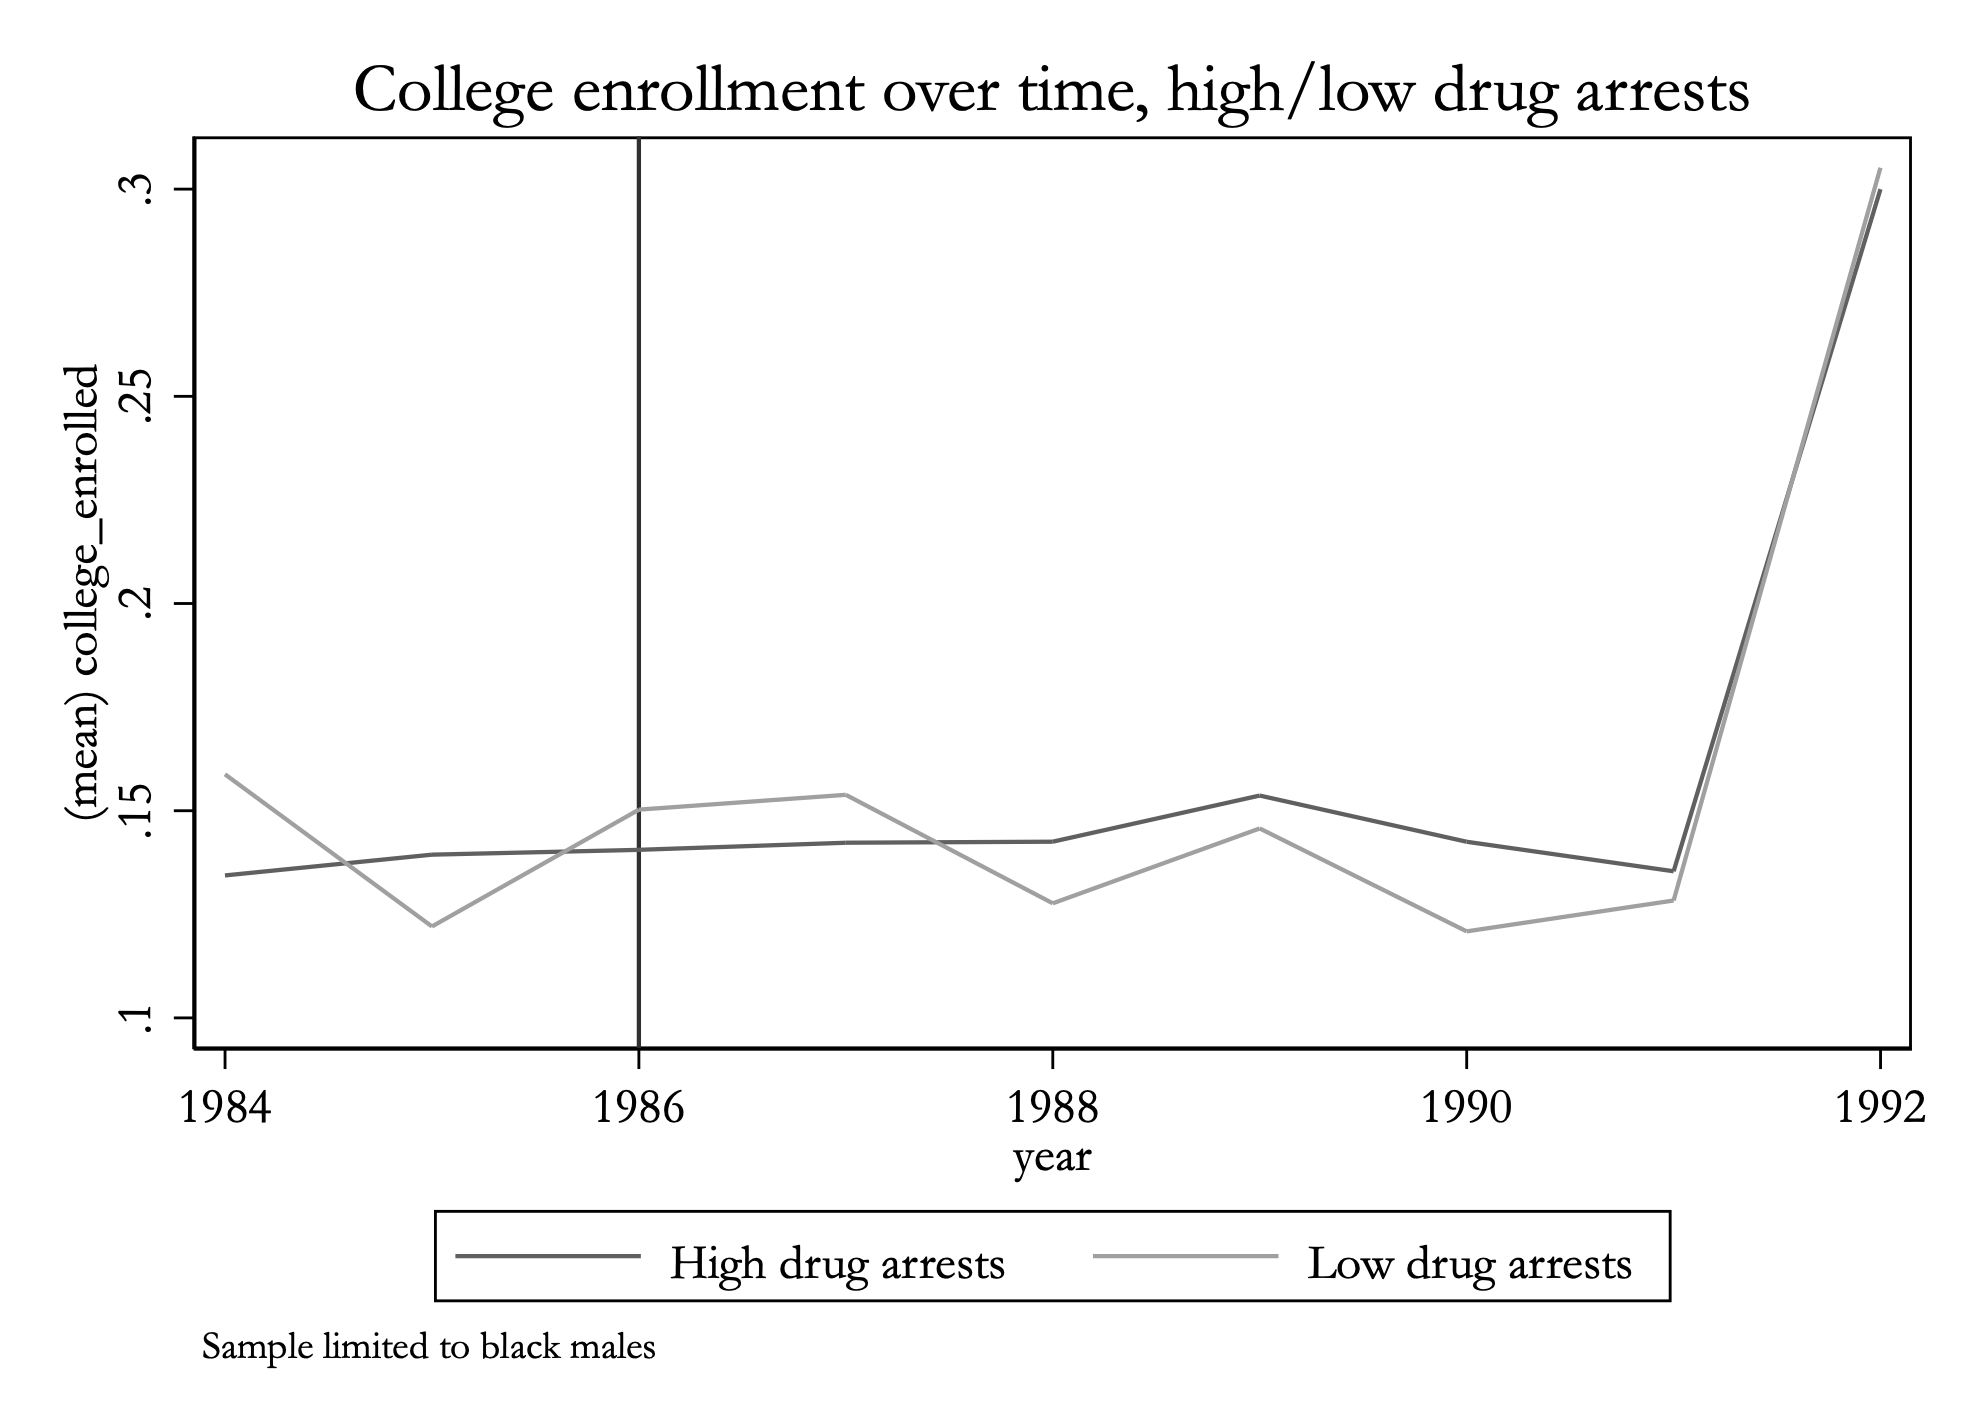
\includegraphics[width=7cm]{pretrends/1986/college_enroll_bydrugarrests_1986.png} }}%
    \qquad
    \subfloat[\centering 2010]{{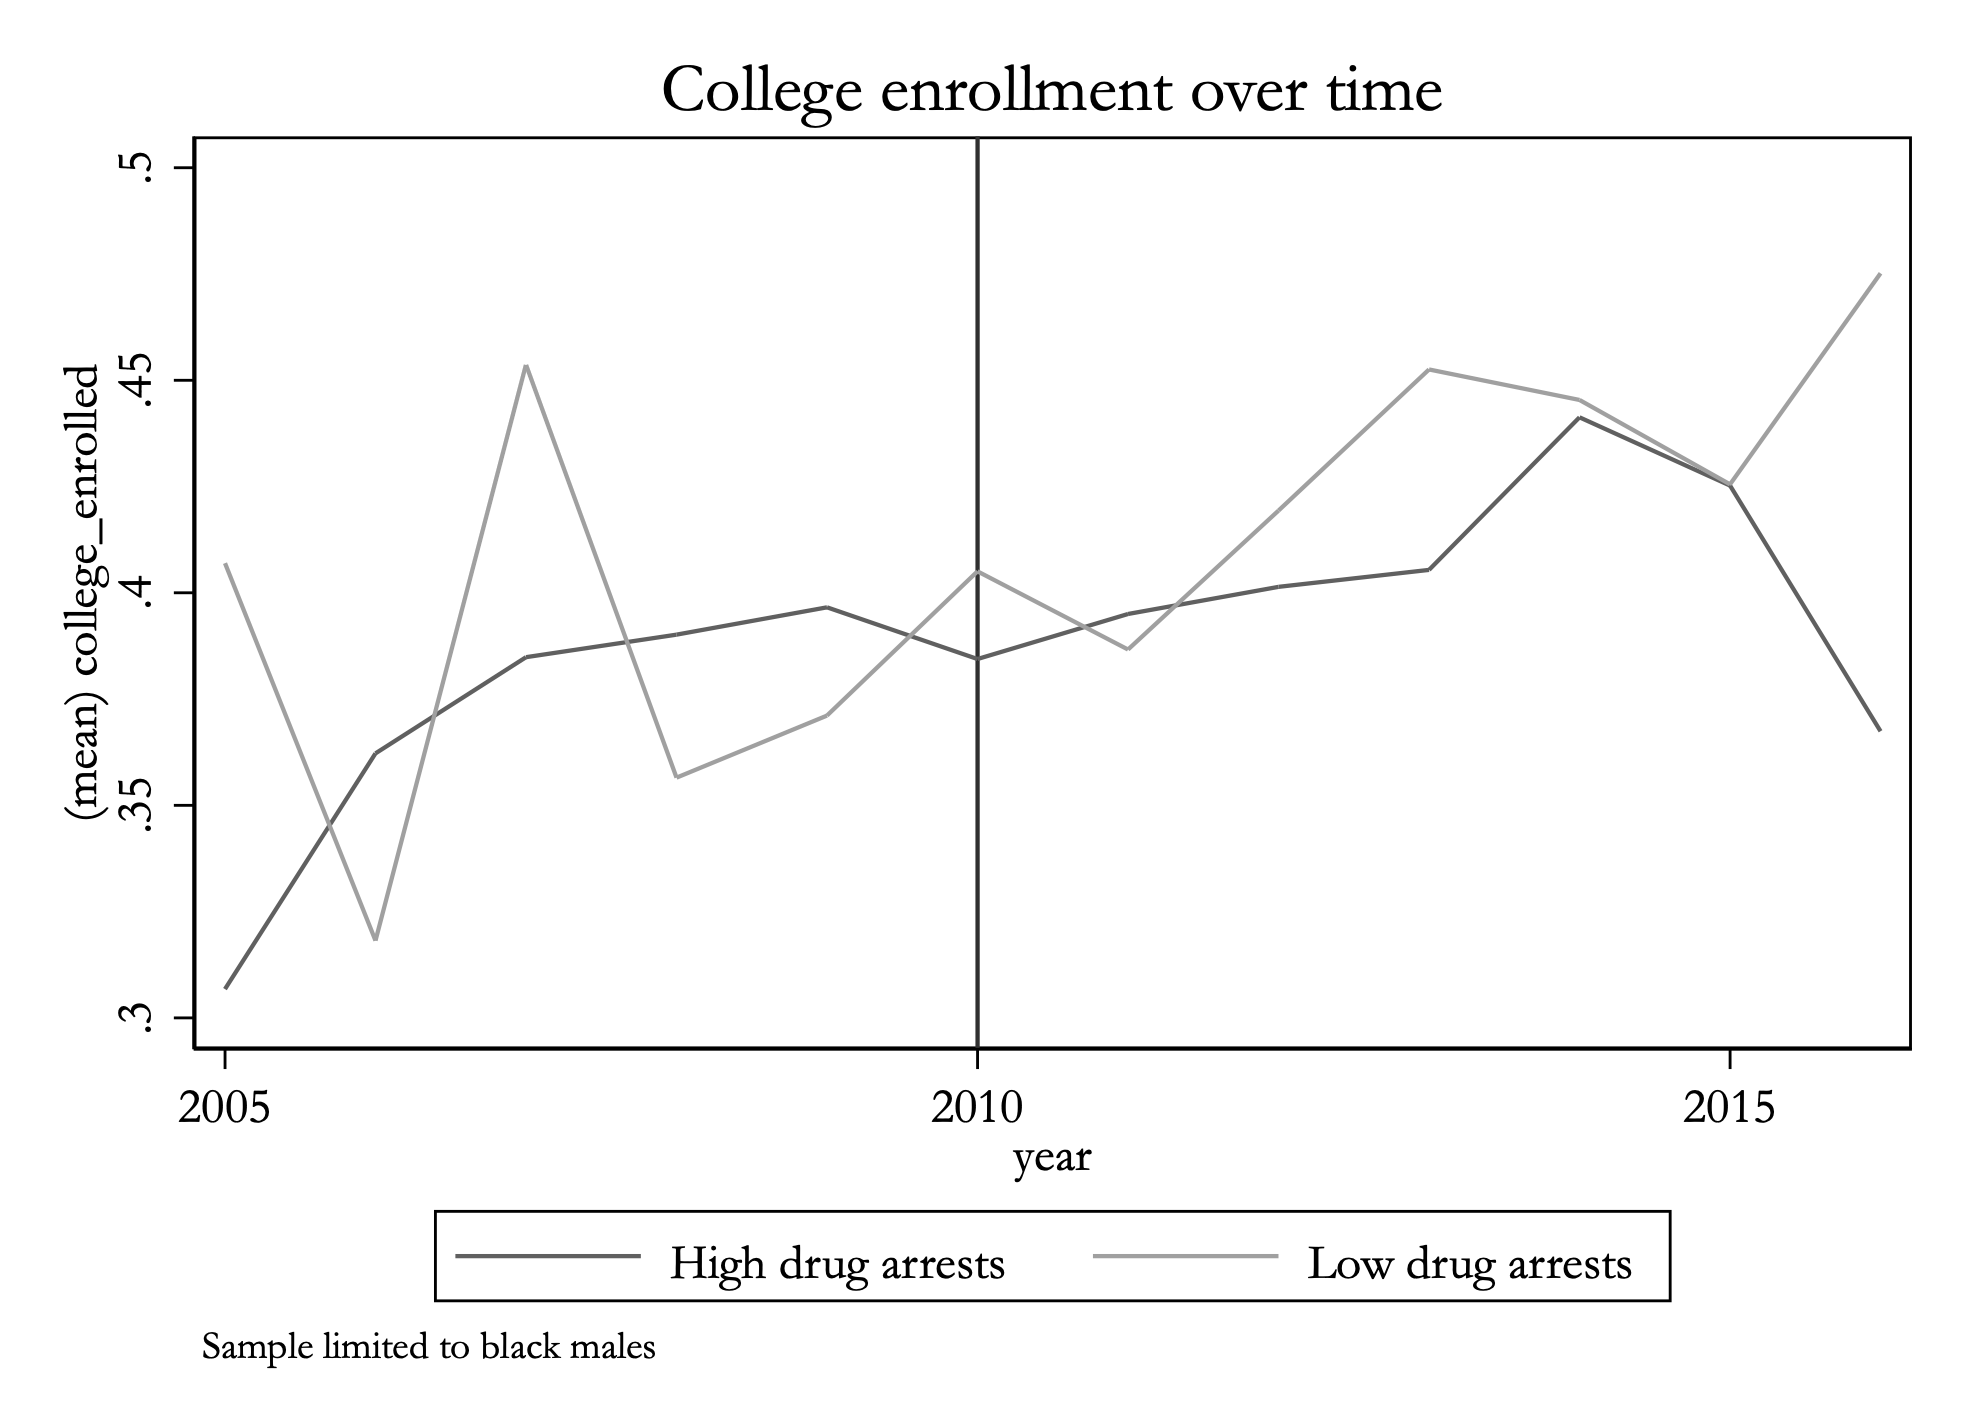
\includegraphics[width=7cm]{pretrends/2010/college_enroll_bydrugarrests_2010.png} }}%
    \label{fig:raw_college_highlowab_1986}%
  \end{figure}
  \begin{figure}[h]
    \centering
    \caption{College Enrollment By States with High vs Low Black Juvenile Drug Arrest Rates}%
    \subfloat[\centering 1986]{{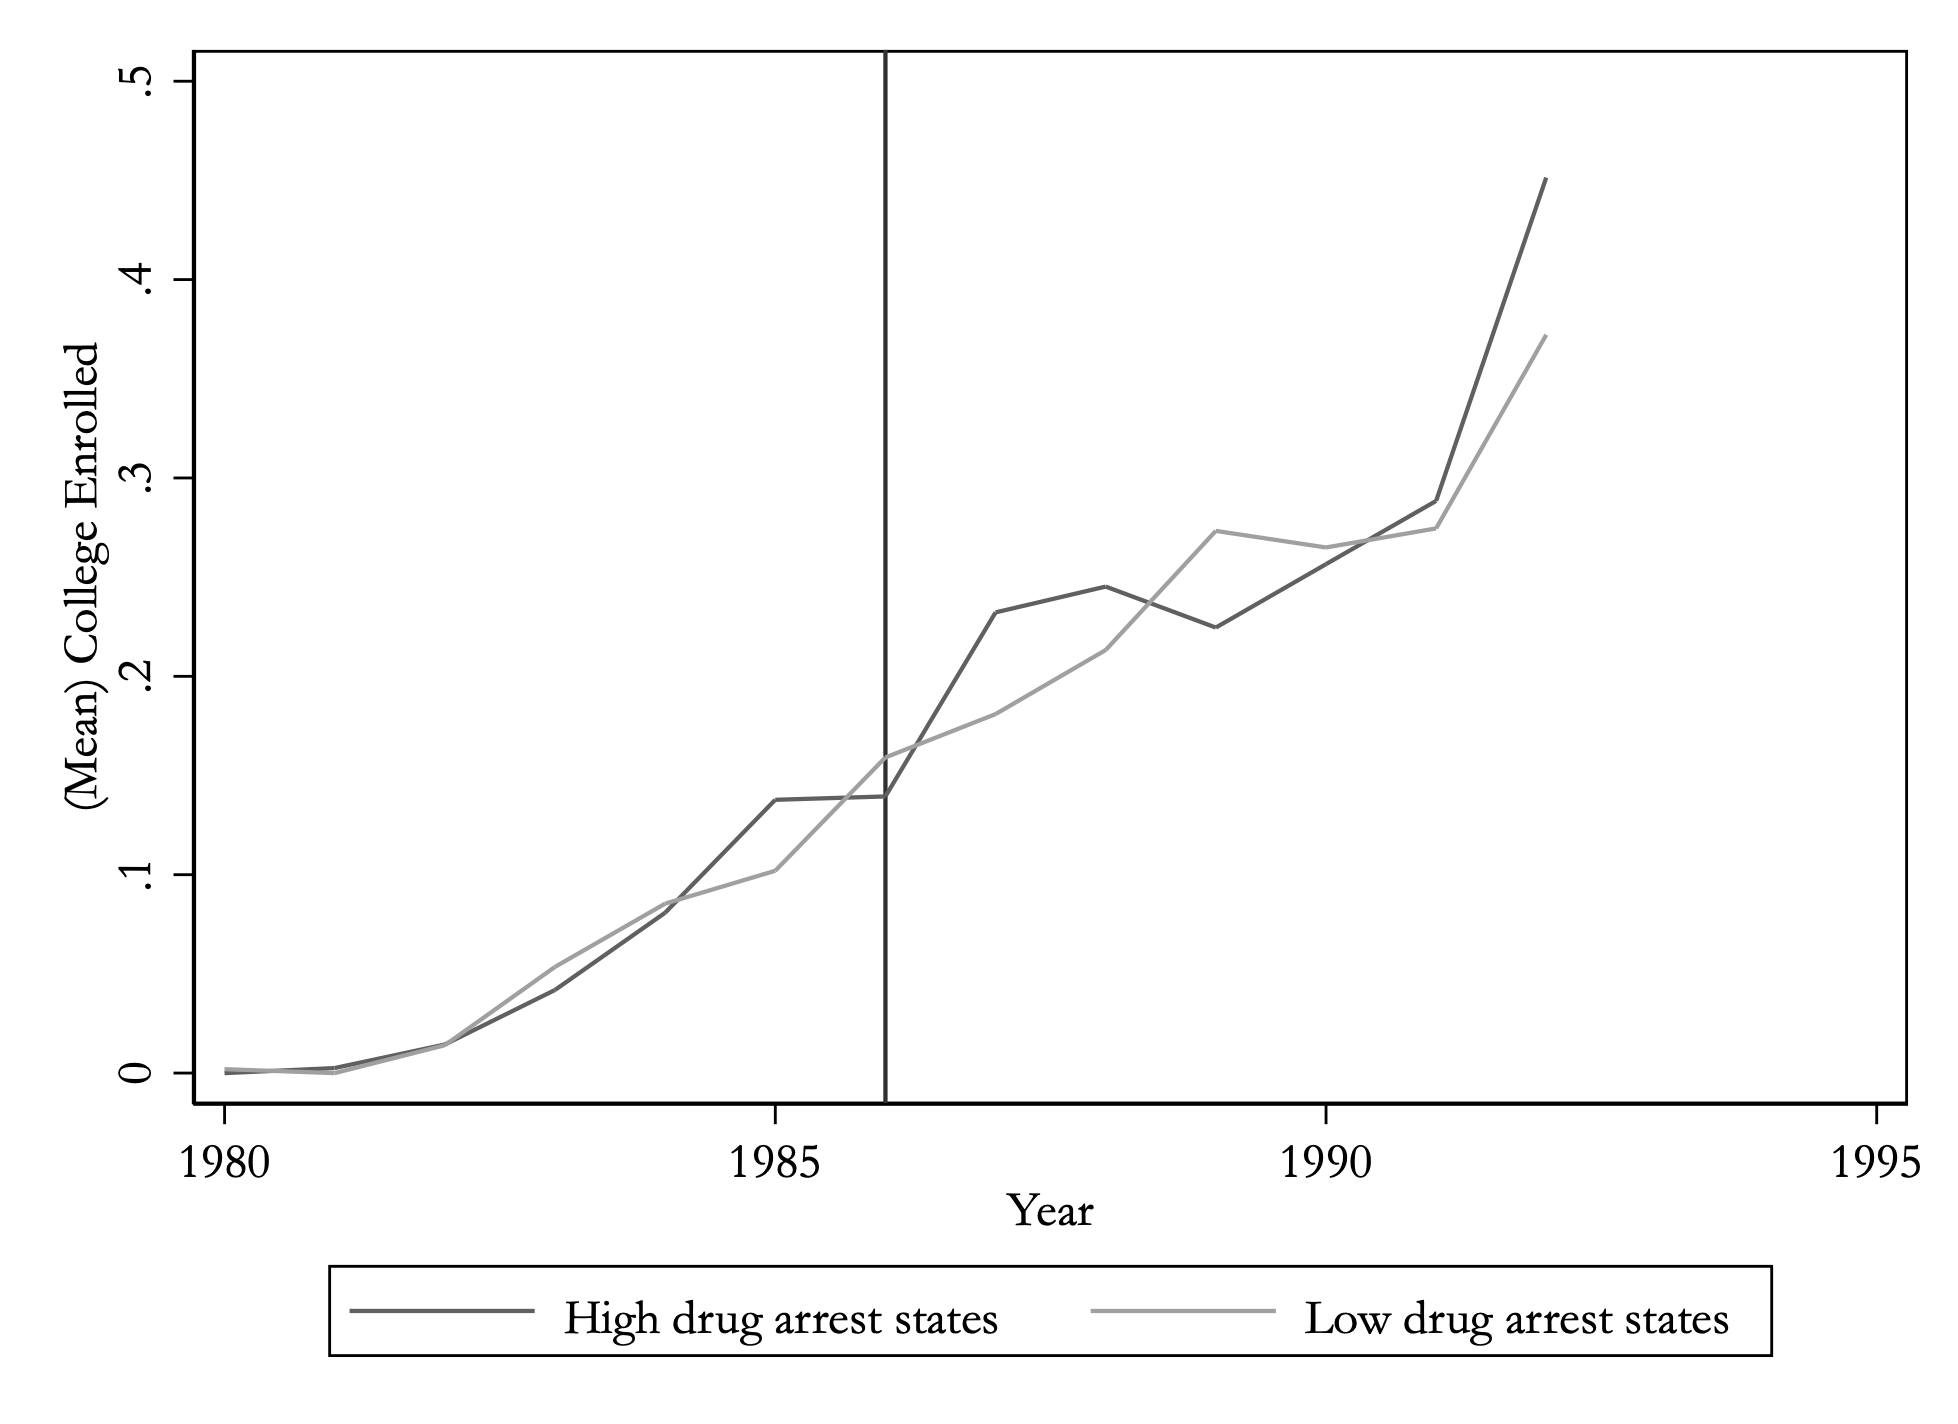
\includegraphics[width=7cm]{pretrends/1986/college_enroll_bydrugarrests_jb_1986.png} }}%
    \qquad
    \subfloat[\centering 2010]{{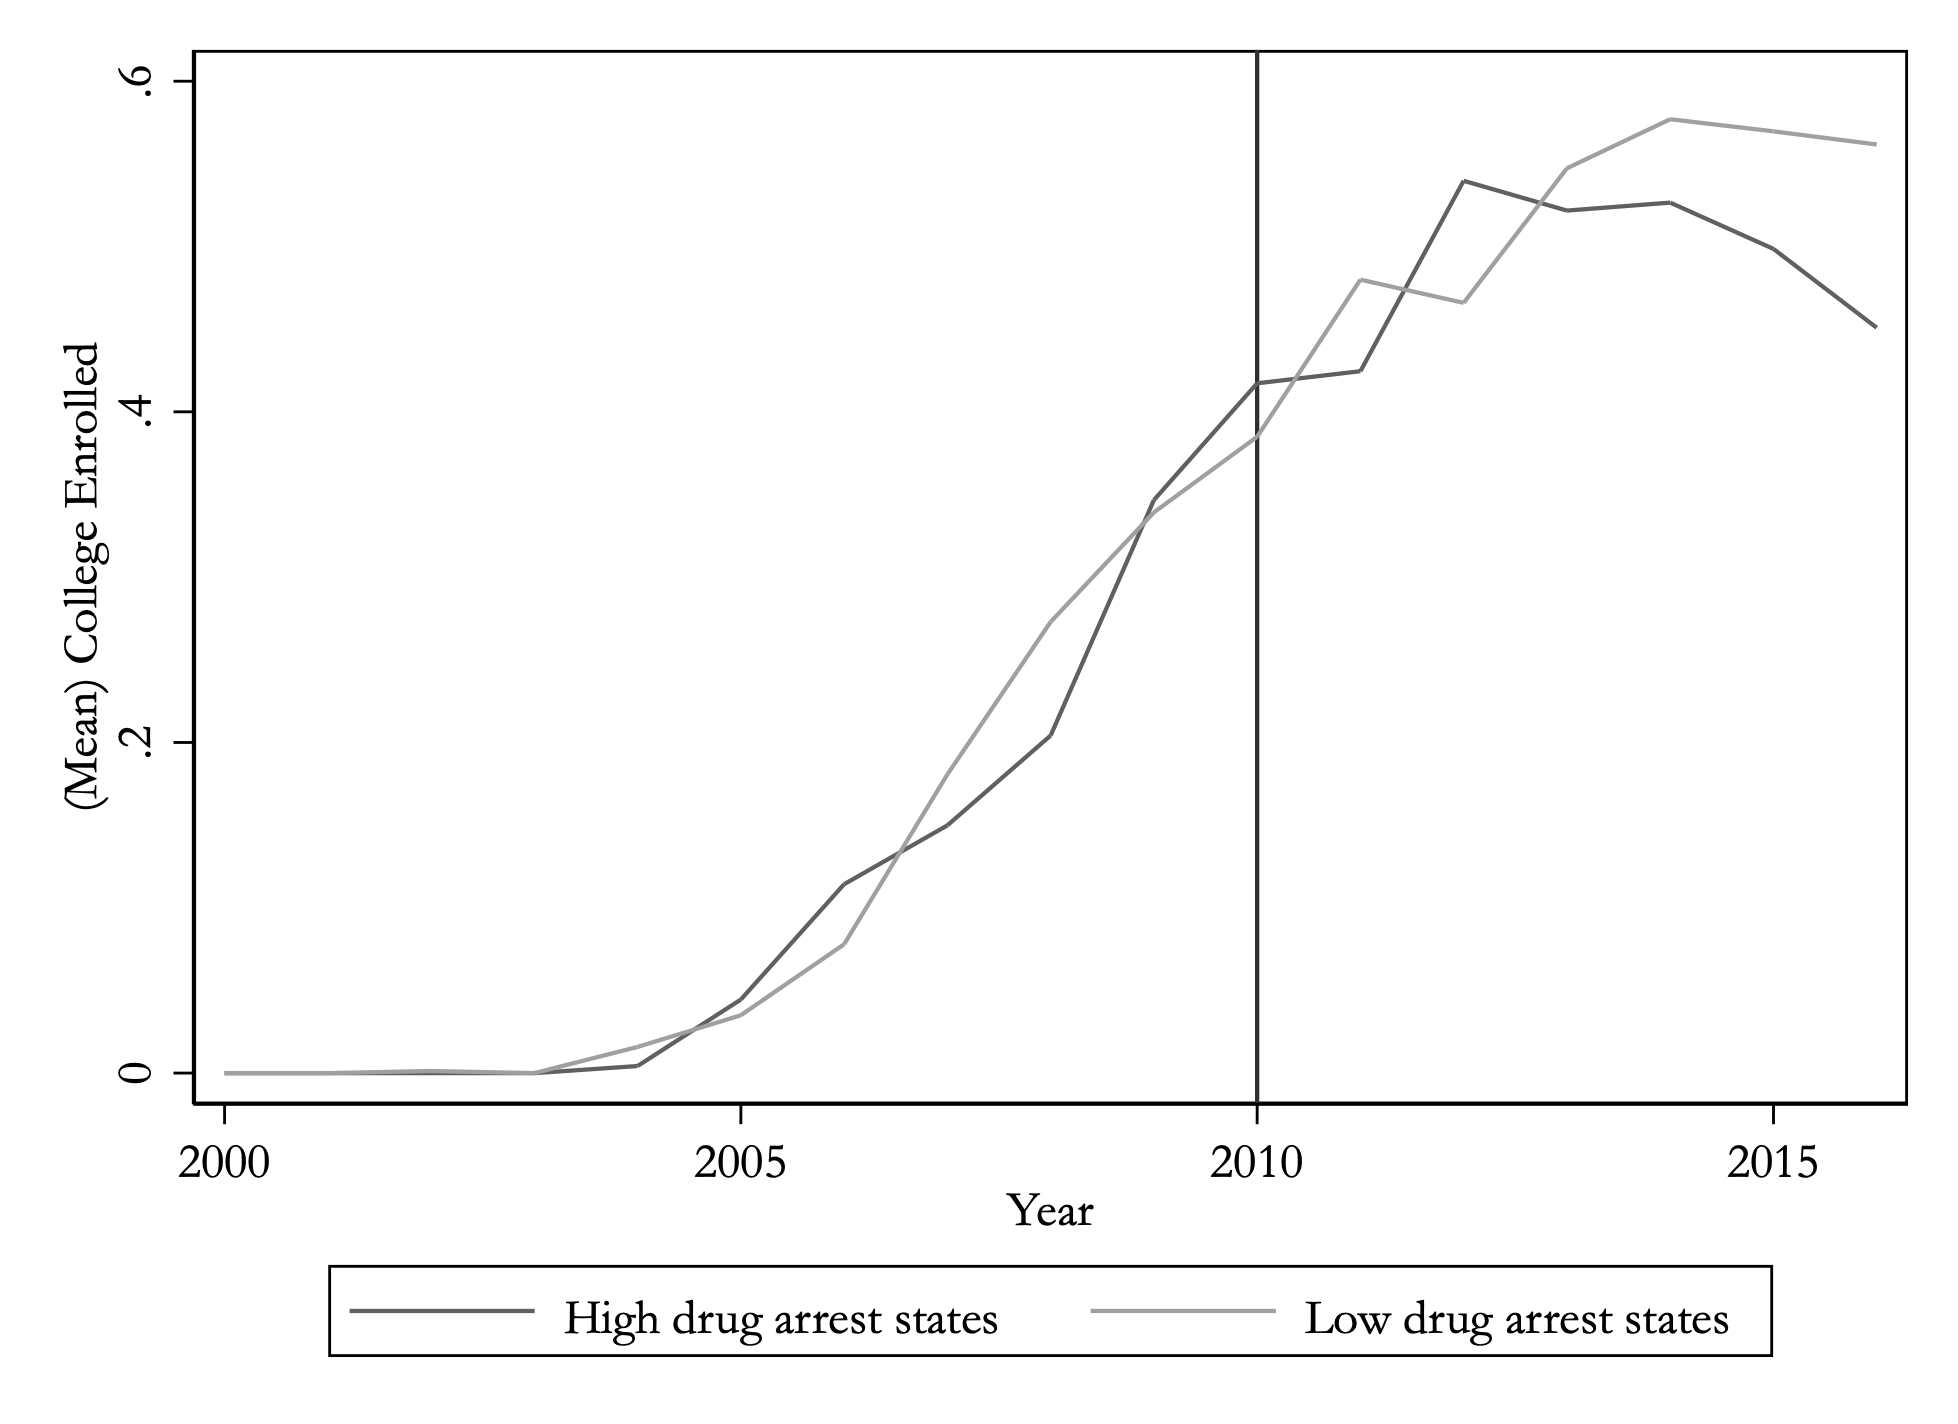
\includegraphics[width=7cm]{pretrends/2010/college_enroll_bydrugarrests_jb_2010.png} }}%
    \label{fig:raw_college_highlowjb_1986}%
  \end{figure}
  
  \begin{footnotesize}
    \noindent Note: These figures report the proportion enrolled in college plotted over time using CPS data from 1984-1992 and 2005-2016 for high black adult/juvenile drug arrest states and low black adult/juvenile drug arrest states, where high black adult/juvenile drug arrest states are defined to be those above the 75th percentile in 1984 and 2008. A vertical line is drawn to denote the passage of the Anti-Drug Abuse Act of 1986 and the Fair Sentencing Act of 2010. The sample is defined as black males aged 18-24 in 1986 and 2010 who were not incarcerated at the time of the survey.
  \end{footnotesize}
  
  \clearpage

  \begin{figure}[h]
    \caption{Black Adult Drug-related Arrest Rate Per 100,000 in 1984} 
    \centering
    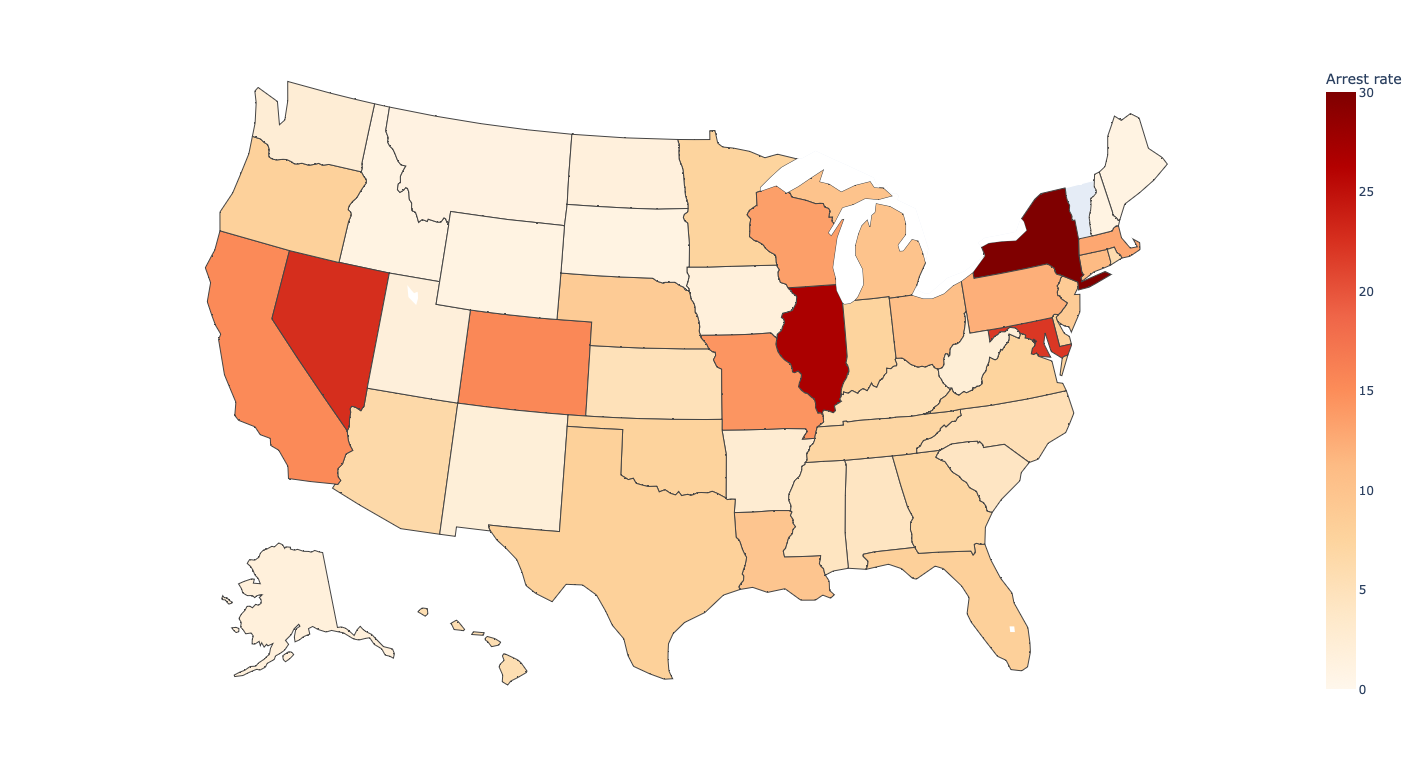
\includegraphics[width=0.8\textwidth]{heatmap/ab1986.png}
    \label{fig:heatmap}
  \end{figure}
  
  \begin{footnotesize}
    \noindent Note: This figure presents a heatmap of the United States at the state level using UCR Program data. The data is from 1984, and I use all drug-related arrests for Black adult men. Although New York's normalized arrest rate is at 48, I capped the maximum at 30 for clarity of states with low normalized drug arrest rates, since the distribution is heavily right-skewed. High drug arrest states are defined as states above the 75th percentile, and the 75th percentile is at 17.4 Black adult arrests per 100,000.
  \end{footnotesize}
  
  \vspace*{8mm}
  
  \begin{figure}[h]
    \centering
    \caption{Distribution of Black Adult Drug-Related Arrest Rates}%
    \subfloat[\centering 1984]{{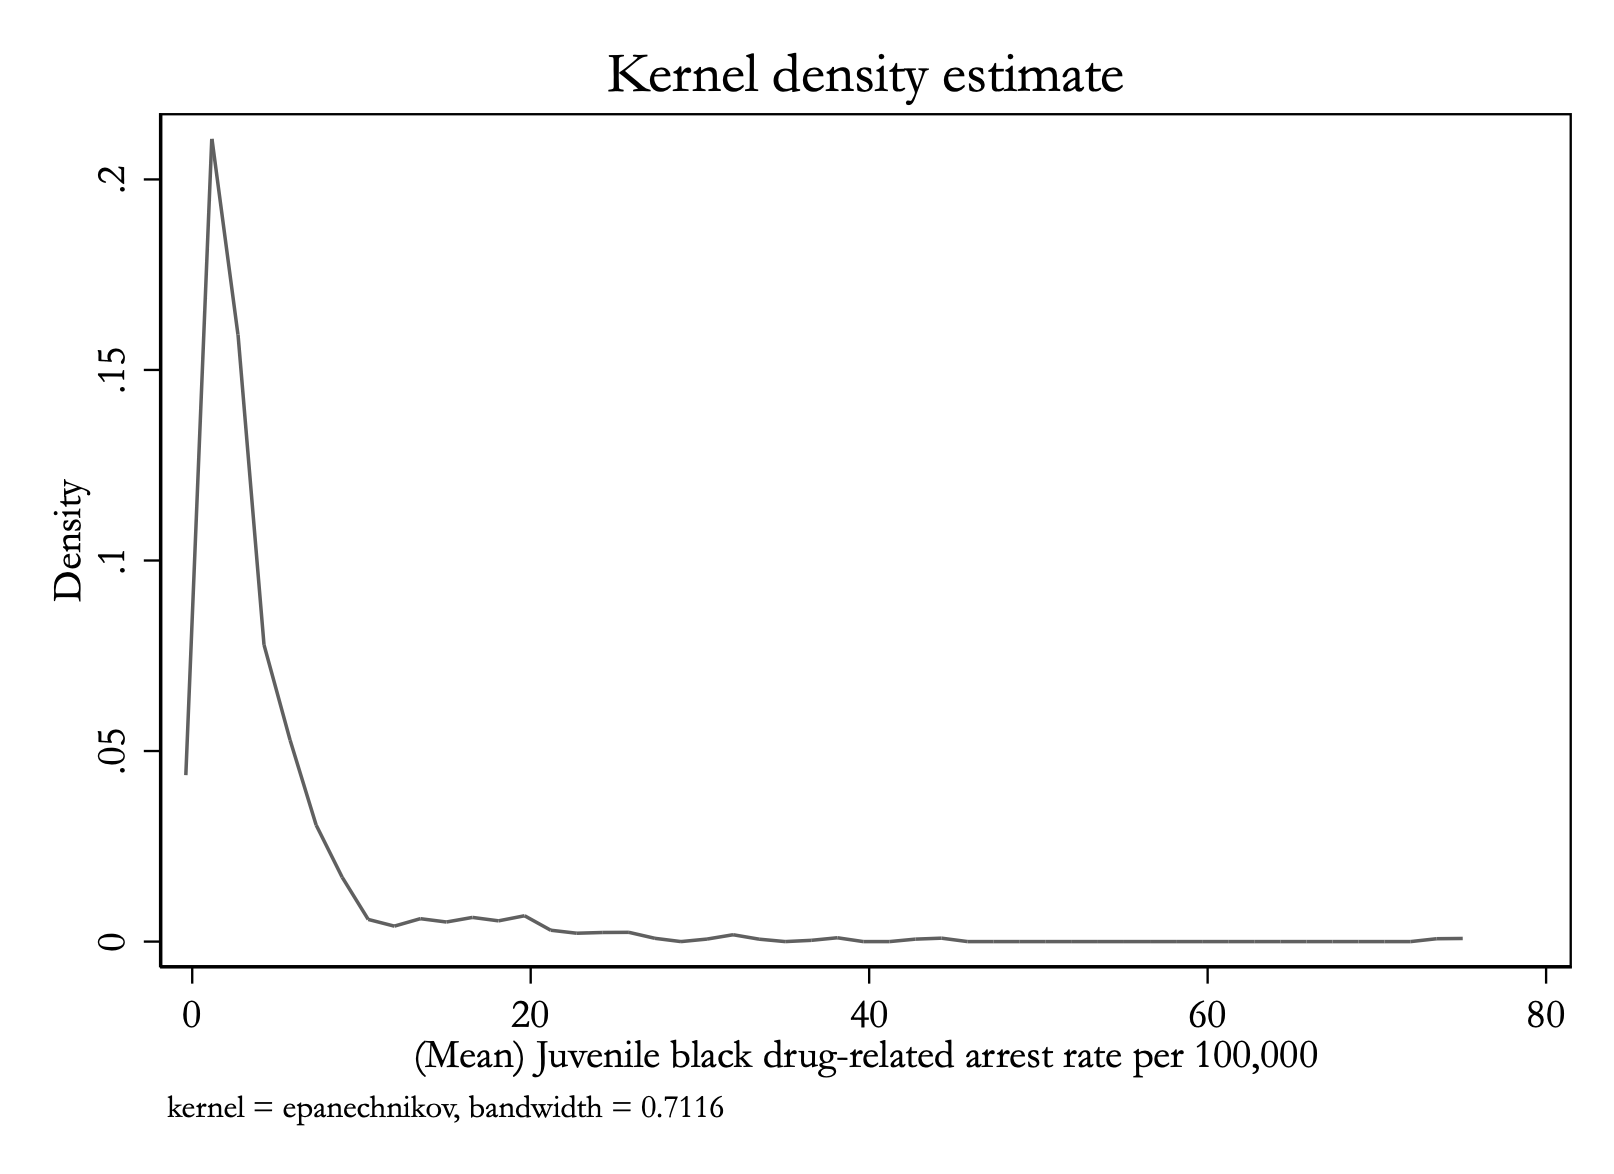
\includegraphics[width=7cm]{descriptive/norm_jb_100000_density_1986} }}%
    \qquad
    \subfloat[\centering 2008]{{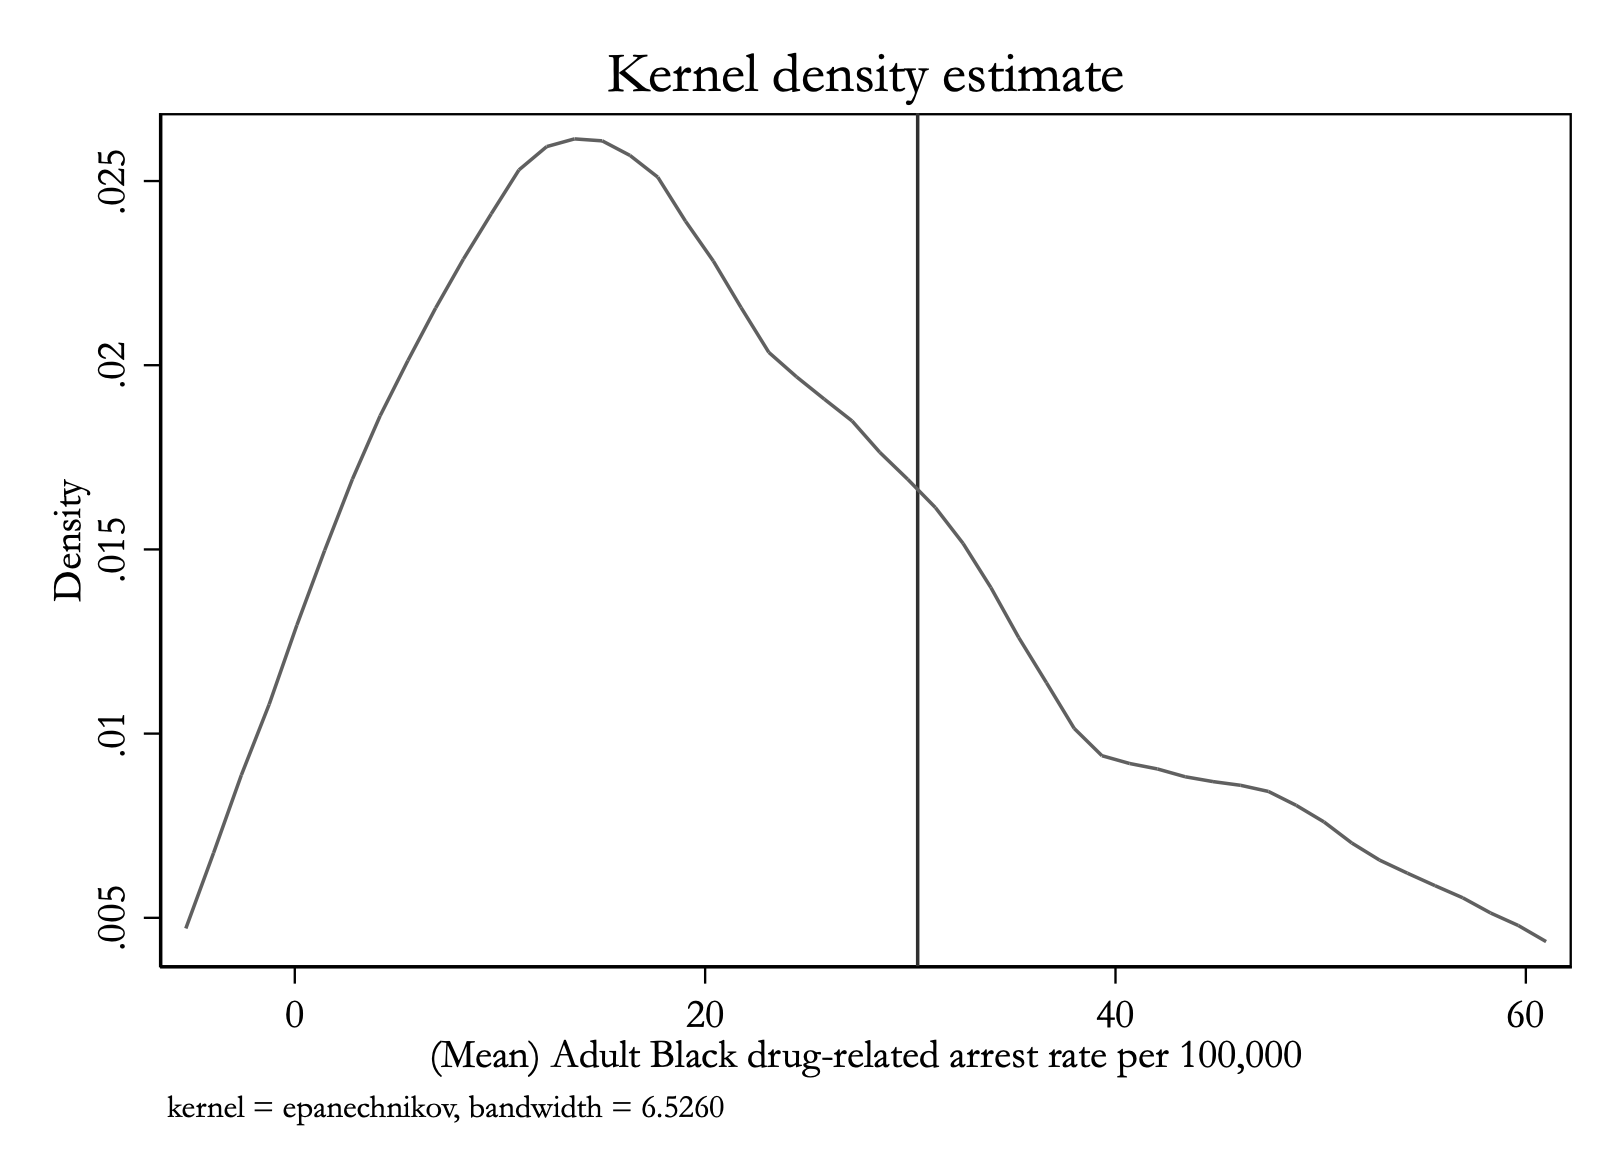
\includegraphics[width=7cm]{descriptive/norm_jb_100000_density_2010.png} }}%
    \label{fig:density_jb}%
  \end{figure}
  \begin{footnotesize}
    \noindent Note: These figures report the kernel density estimates for the normalized drug-related Black adult arrest rate in 1984 and 2008. The vertical line denotes the 75th percentile. Right tail outliers were winsorized at the 95\% level for both figures.
  \end{footnotesize}
  
  \clearpage
     

  % Event study
  \begin{figure}[h]
    \caption{Effect of Anti-Drug Abuse Act on Drug-related Arrest Rate of Adult Black Men, Comparing States with High and Low Black Adult Drug-Related Arrest Rates (with Fixed Effects)}
    \centering
    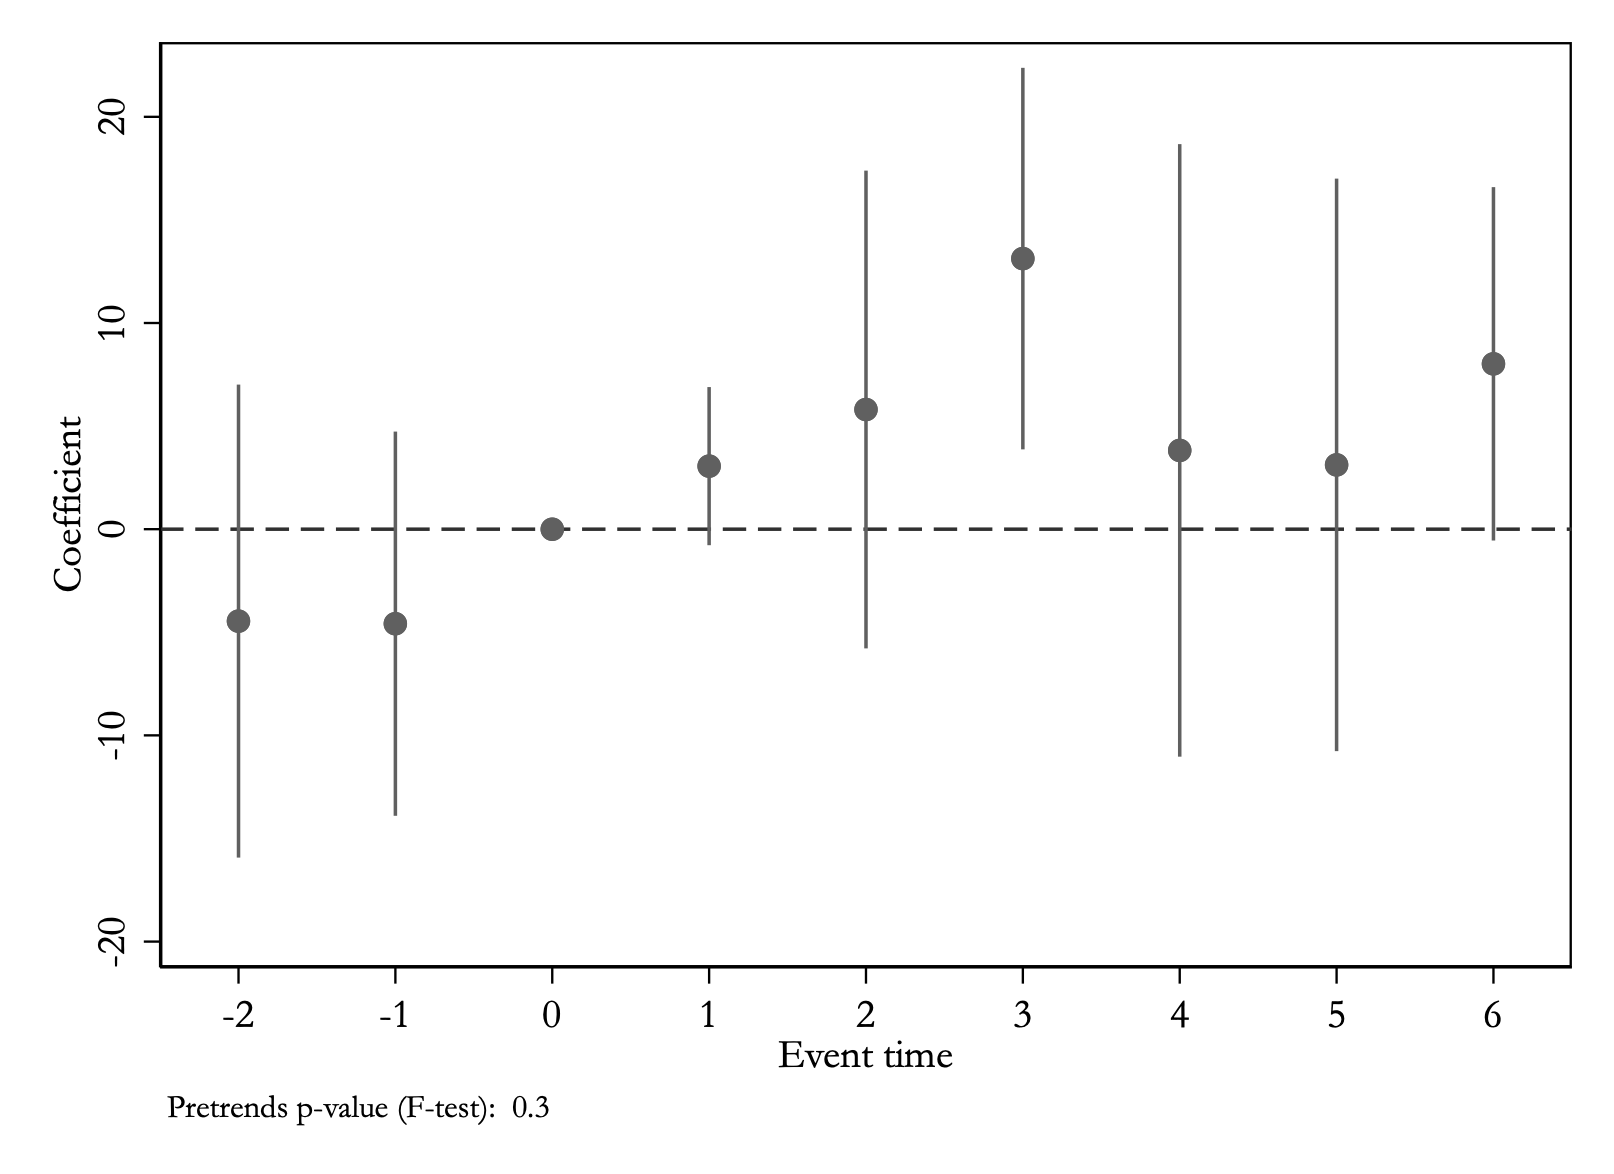
\includegraphics[width=0.7\textwidth]{eventstudy/high_drug_use/high_drug_eventstudy_1986.png}
    \label{fig:ab_es_1986}
  \end{figure}

  \begin{figure}[H]
    \caption{Effect of Anti-Drug Abuse Act on Drug-related Arrest Rate of Adult Black Men, Comparing States with High and Low Black Adult Drug-Related Arrest Rates (without Fixed Effects)}
    \centering
    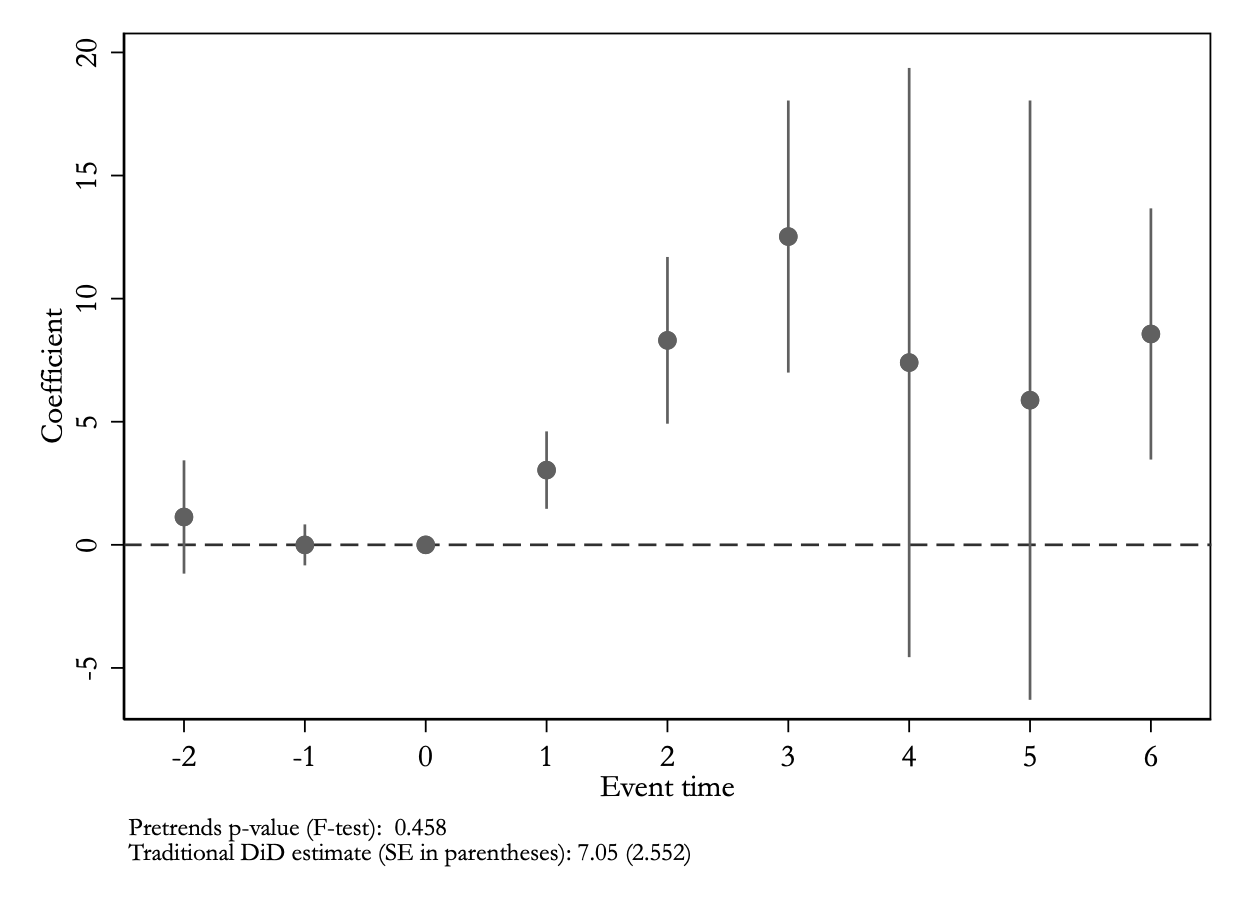
\includegraphics[width=0.7\textwidth]{eventstudy/high_drug_use/high_drug_eventstudy_nofe_1986.png}
    \label{fig:ab_es_1986_nofe}
  \end{figure}
  
  \begin{footnotesize}
    \noindent Note: This figure reports coefficients from the estimation of equation \ref{eq:state_level_es} evaluating the impact of the Anti-Drug Abuse Act of 1986 on arrest rates per 100,000 related to drug violations using CPS and UCR data from 1982-1992. Event time $0 \coloneqq 1986$. The coefficients represent the change in outcomes for high-drug arrest states relative to non-high-drug arrest states, where high black adult drug arrest states are defined to be those above the 75th percentile in 1984. The sample is defined as black males aged 18-24 in 1986 who were not incarcerated at the time of the survey. Control variables include population and unemployment rates at the state-year level. Right tail arrest rate outliers were winsorized at the 95\% level.
  \end{footnotesize}
  
  \clearpage

  \begin{figure}[h]
    \caption{Effect of Anti-Drug Abuse Act on Drug-related Arrest Rate of Black Men, Comparing States with High and Low Black Juvenile Drug-Related Arrest Rate}
    \centering
    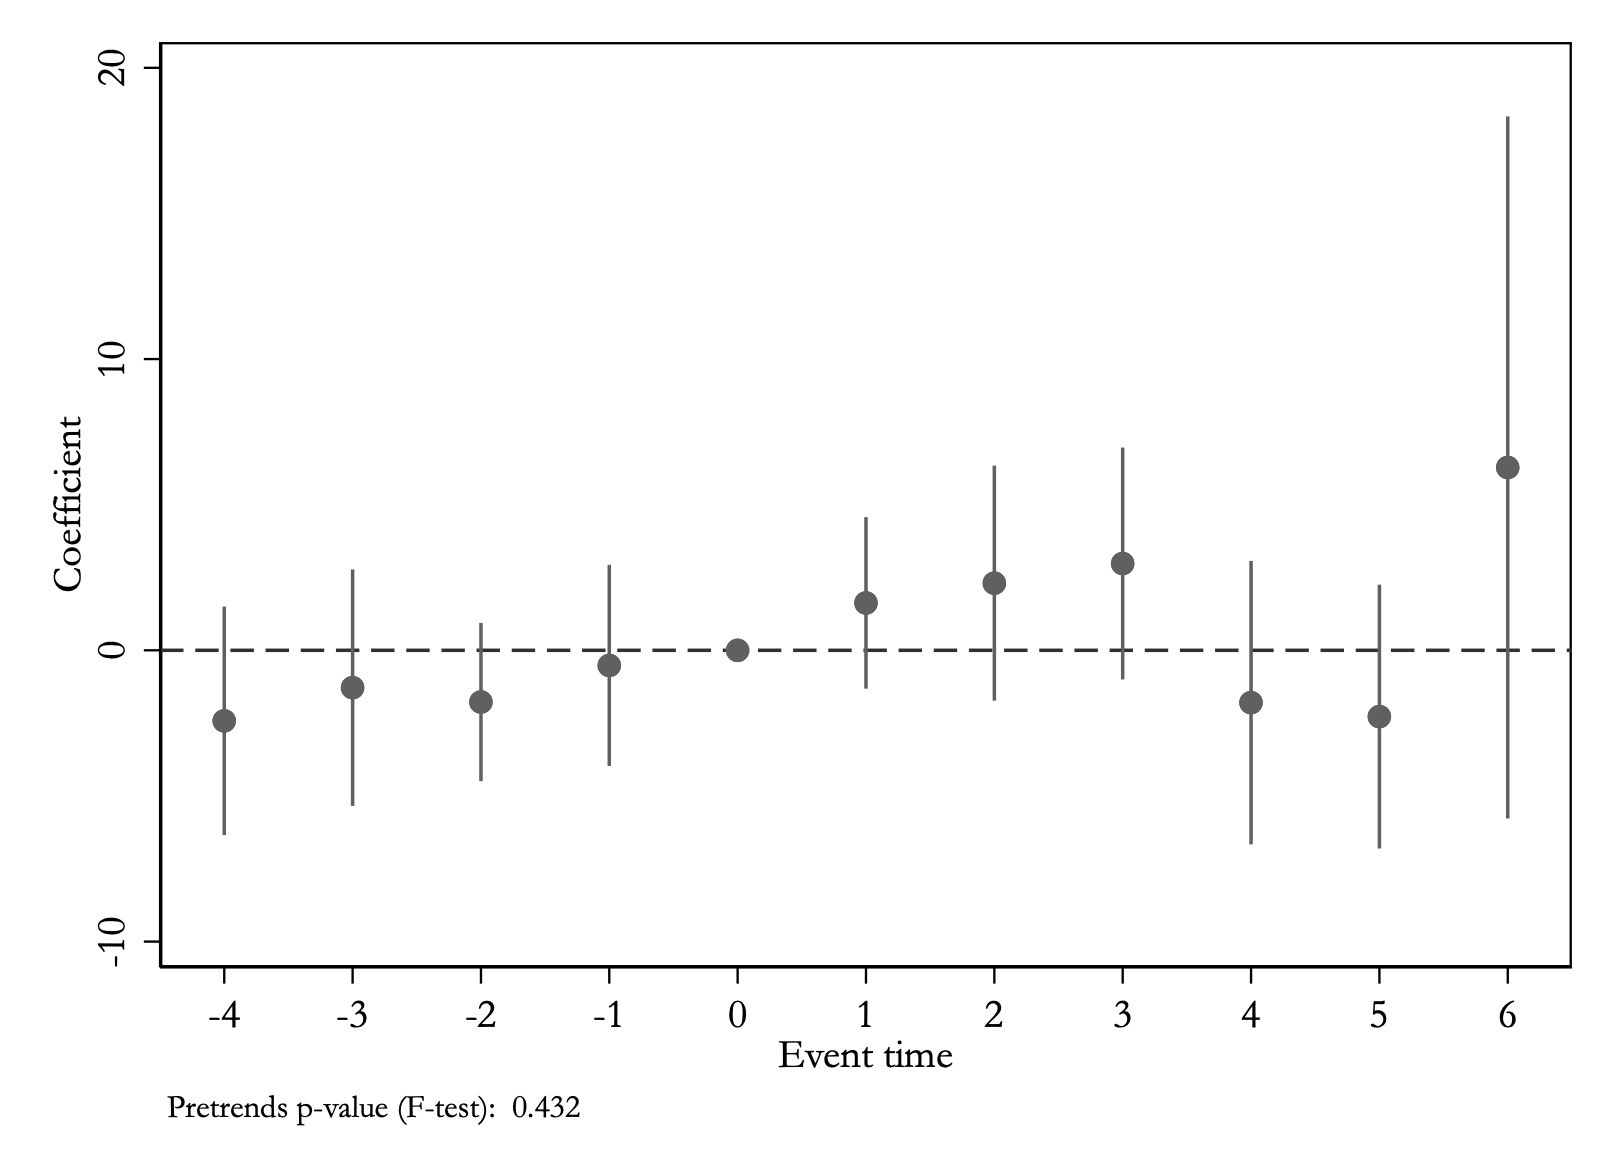
\includegraphics[width=1\textwidth]{eventstudy/high_drug_use/high_drug_eventstudy_1986_jb.png}
    \label{fig:jb_es_1986}
  \end{figure}

  \begin{footnotesize}
    \noindent Note: This figure reports coefficients from the estimation of equation 1 evaluating the impact of the Anti-Drug Abuse Act of 1986 on arrest rates per 100,000 related to drug violations using CPS and UCR data from 1982-1992. Event time $0 \coloneqq 1986$. The coefficients represent the change in outcomes for high black juvenile drug arrest states relative to non-high-drug arrest states, where high-drug arrest states are defined to be those above the 75th percentile in 1984. The sample is defined as black males aged 18-24 in 1986 who were not incarcerated at the time of the survey. Control variables include population and unemployment rates at the state-year level. 
  \end{footnotesize}

  \clearpage

  \begin{figure}[h]
    \centering
    \caption{Additional Pretrend Testing for Coefficients from Figure 7}%
    \subfloat[\centering Linear pretrend]{{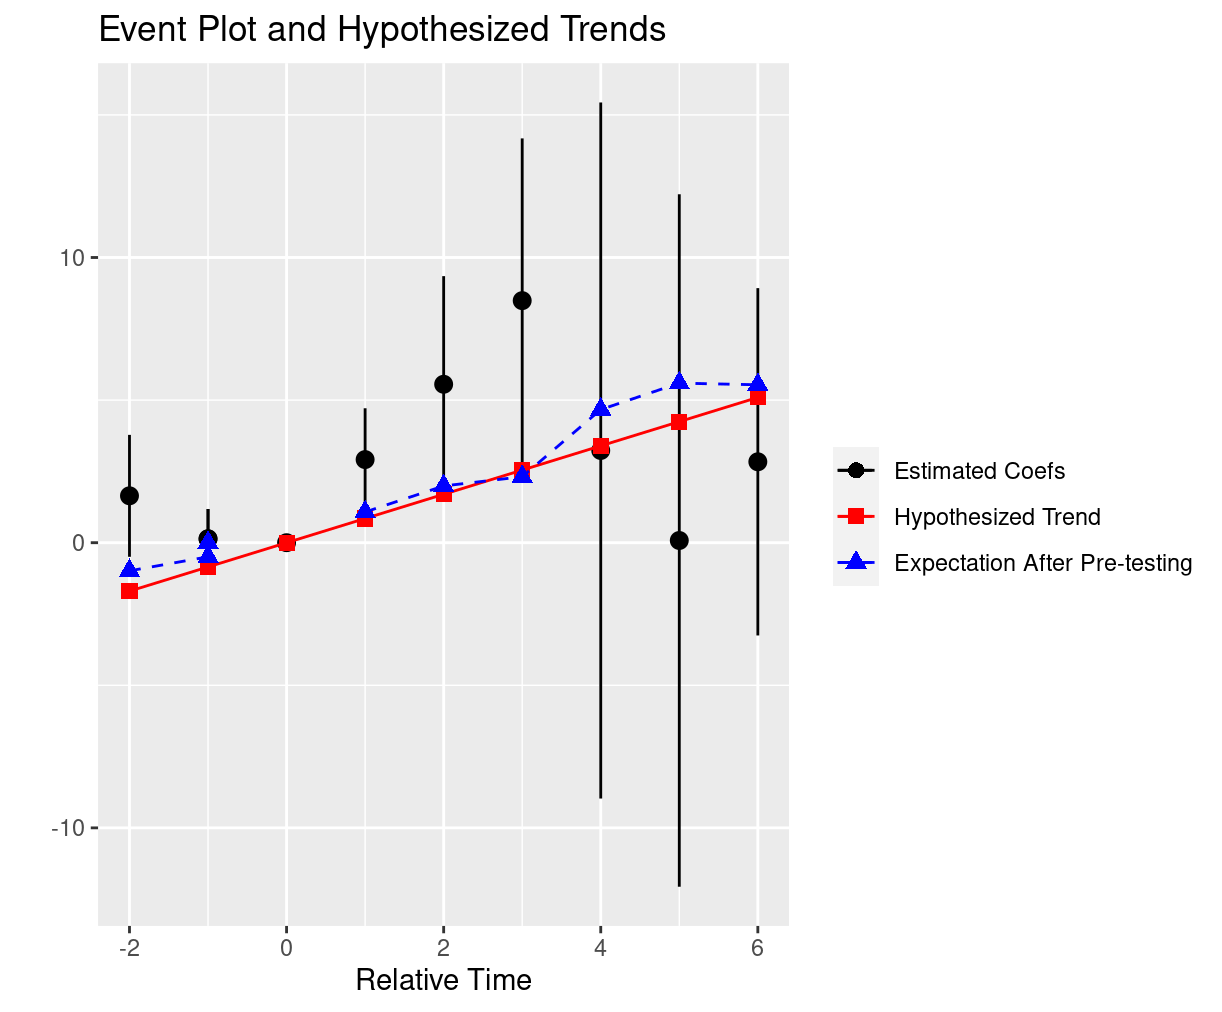
\includegraphics[width=7cm]{pretrends/power/firststage_linear_ab1986.png} }}%
    \qquad
    \subfloat[\centering Quadratic pretrend]{{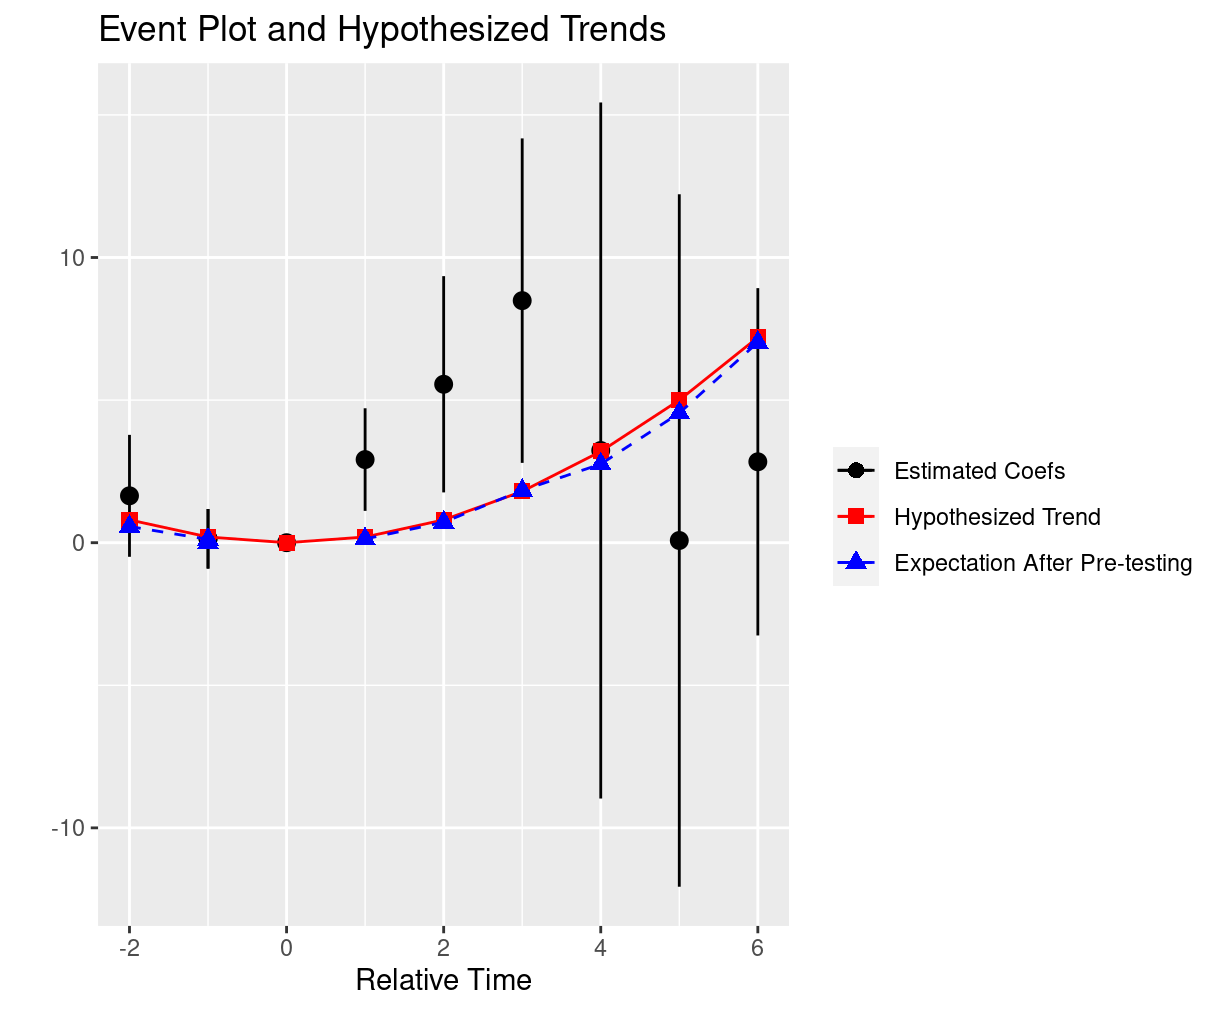
\includegraphics[width=7cm]{pretrends/power/firststage_quad_ab1986.png} }}%
    \label{fig:pretrends_roth}%
  \end{figure}

  \begin{footnotesize}
    \noindent Note: These two figures were constructed using an R package written by \cite{roth2022}. The figures and pretrend statistics were calculated using the estimated coefficients from Figure 7 and their corresponding covariance matrixes. The slope in Figure A was constructed such that the power would be about 0.5, while the quadratic trend in Figure B was chosen visually.

    Figure A statistics: 1) power = 0.499, 2) Bayes Factor = 0.549, 3) likelihood ratio = 0.033.

    Figure B statistics: 1) power = 0.155, 2) Bayes Factor = 0.928, 3) likelihood ratio = 2.323.
  \end{footnotesize}

  \clearpage
  
  \begin{figure}[h]
    \centering
    \caption{Effect of Fair Sentencing Act on Drug-related Arrest Rate of Adult Black Men, Comparing High and Low-Intensity States}%
    \subfloat[\centering Using adults arrests]{{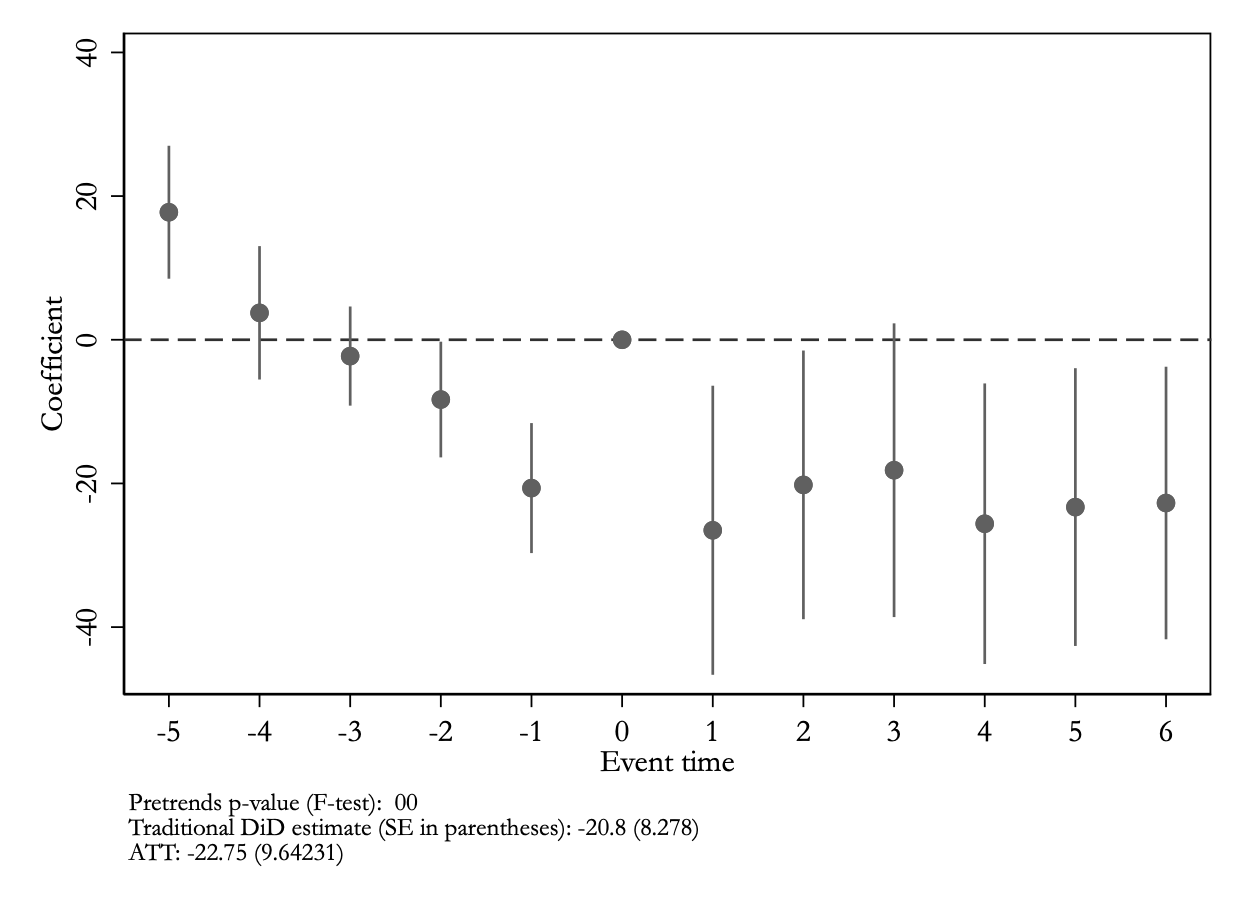
\includegraphics[width=7cm]{eventstudy/high_drug_use/high_drug_eventstudy_2010_ab.png} }}%
    \qquad
    \subfloat[\centering Using juvenile arrests]{{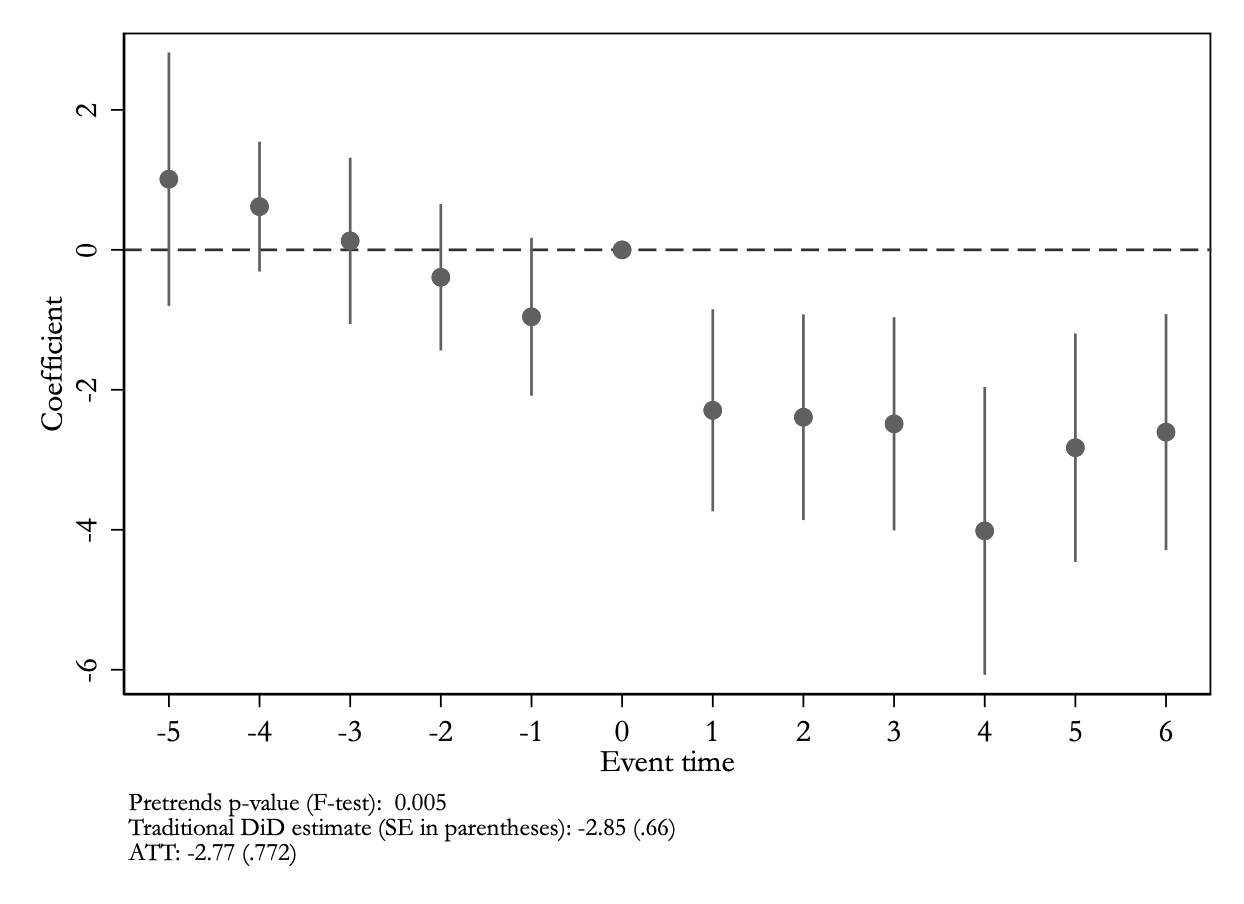
\includegraphics[width=7cm]{eventstudy/high_drug_use/high_drug_eventstudy_2010_jb.png} }}%
    \label{fig:fs_es_2010}%
  \end{figure}


  \begin{footnotesize}
    \noindent Note: These figures report coefficients from the estimation of equation 1 evaluating the impact of the Fair Sentencing Act of 2010 on arrest rates per 100,000 related to drug violations using CPS-UCR merged data from 2005-2015. Figure A defines high-intensity states using Black adult arrests, while Figure B defines high-intensity states using Black juvenile arrests. Event time $0 \coloneqq 2010$. The coefficients represent the change in outcomes for high black adult drug arrest states relative to non-high-drug arrest states, where high-drug arrest states are defined to be those above the 75th percentile in 2008. The sample is defined as black males aged 18-24 in 2010 who were not incarcerated at the time of the survey. Control variables include population and unemployment rates at the state-year level. 
  \end{footnotesize}

\clearpage 

\begin{figure}[h]
  \centering
  \caption{Effect of Fair Sentencing Act on the College Enrollment Rate of Adult Black Men, Comparing High and Low-Intensity States}%
  \subfloat[\centering Using adults arrests]{{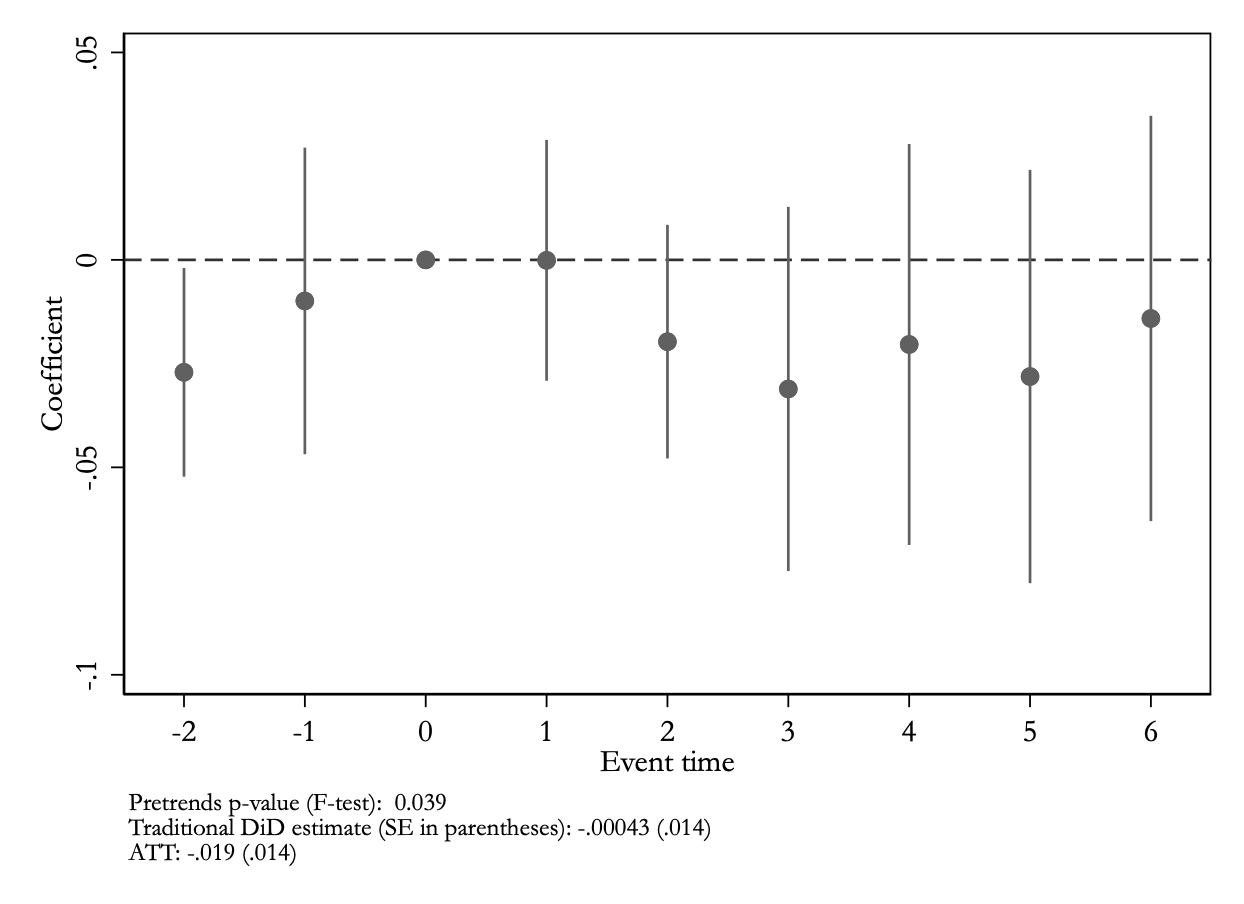
\includegraphics[width=7cm]{eventstudy/high_drug_use/reducedform_ab1986.png} }}%
  \qquad
  \subfloat[\centering Using juvenile arrests]{{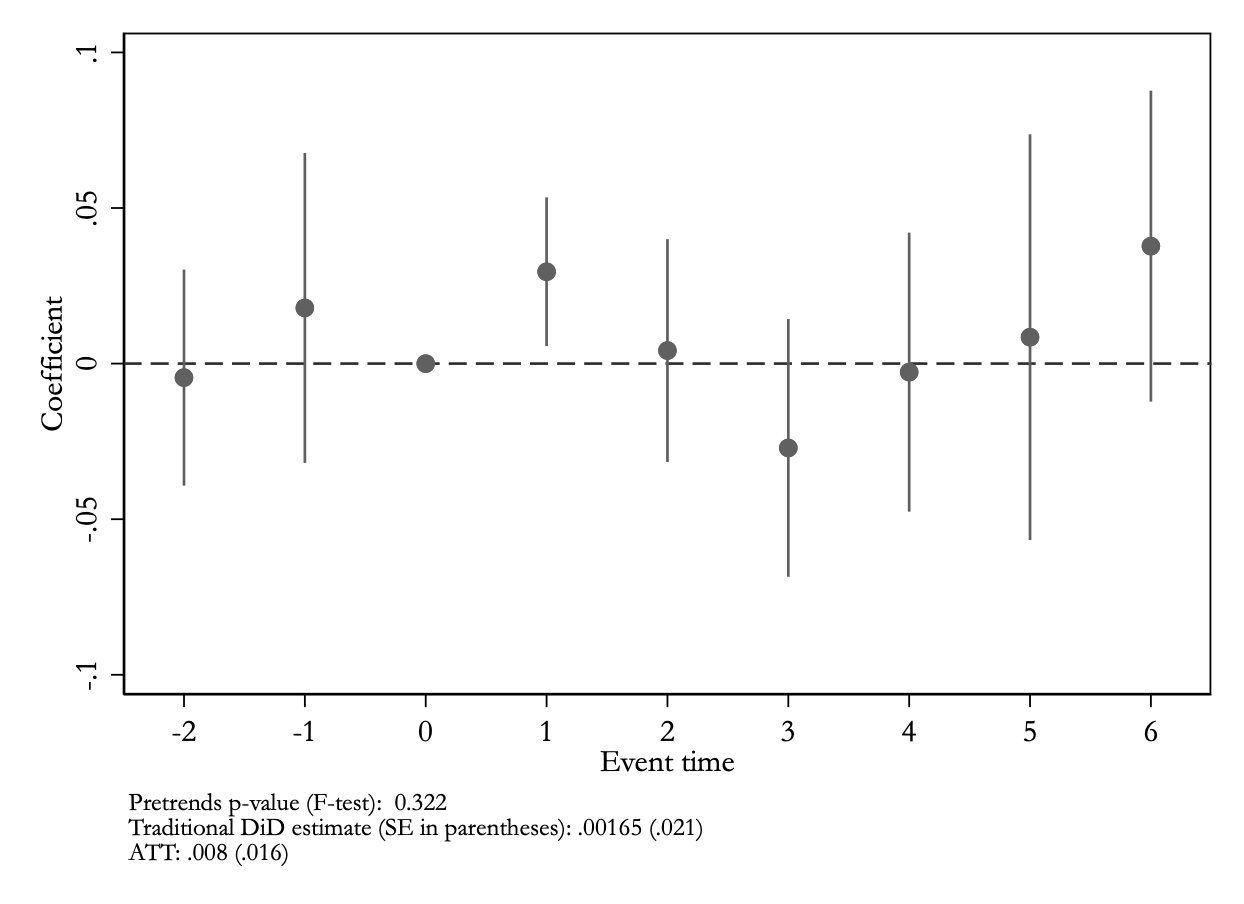
\includegraphics[width=7cm]{eventstudy/high_drug_use/reducedform_jb1986.png} }}%
  \label{fig:rs_es_1986}%
\end{figure}

\begin{footnotesize}
  \noindent Note: These figures report coefficients from the estimation of equation 1 evaluating the impact of the Anti-Drug Abuse Act of 1986 on college enrollment rates using CPS-UCR merged data from 1984-1992. Figure A defines high-intensity states using Black adult arrests, while Figure B defines high-intensity states using Black juvenile arrests. Event time $0 \coloneqq 1986$. The coefficients represent the change in outcomes for high black adult drug arrest states relative to non-high-drug arrest states, where high-drug arrest states are defined to be those above the 75th percentile in 1984. The sample is defined as black males aged 18-24 in 1986 who were not incarcerated at the time of the survey. Control variables include population and unemployment rates at the state-year level. 
\end{footnotesize}

\clearpage

\begin{figure}[h]
  \centering
  \caption{Effect of Fair Sentencing Act on the College Enrollment Rate of Adult Black Men, Comparing High and Low-Intensity States}%
  \subfloat[\centering Using adults arrests]{{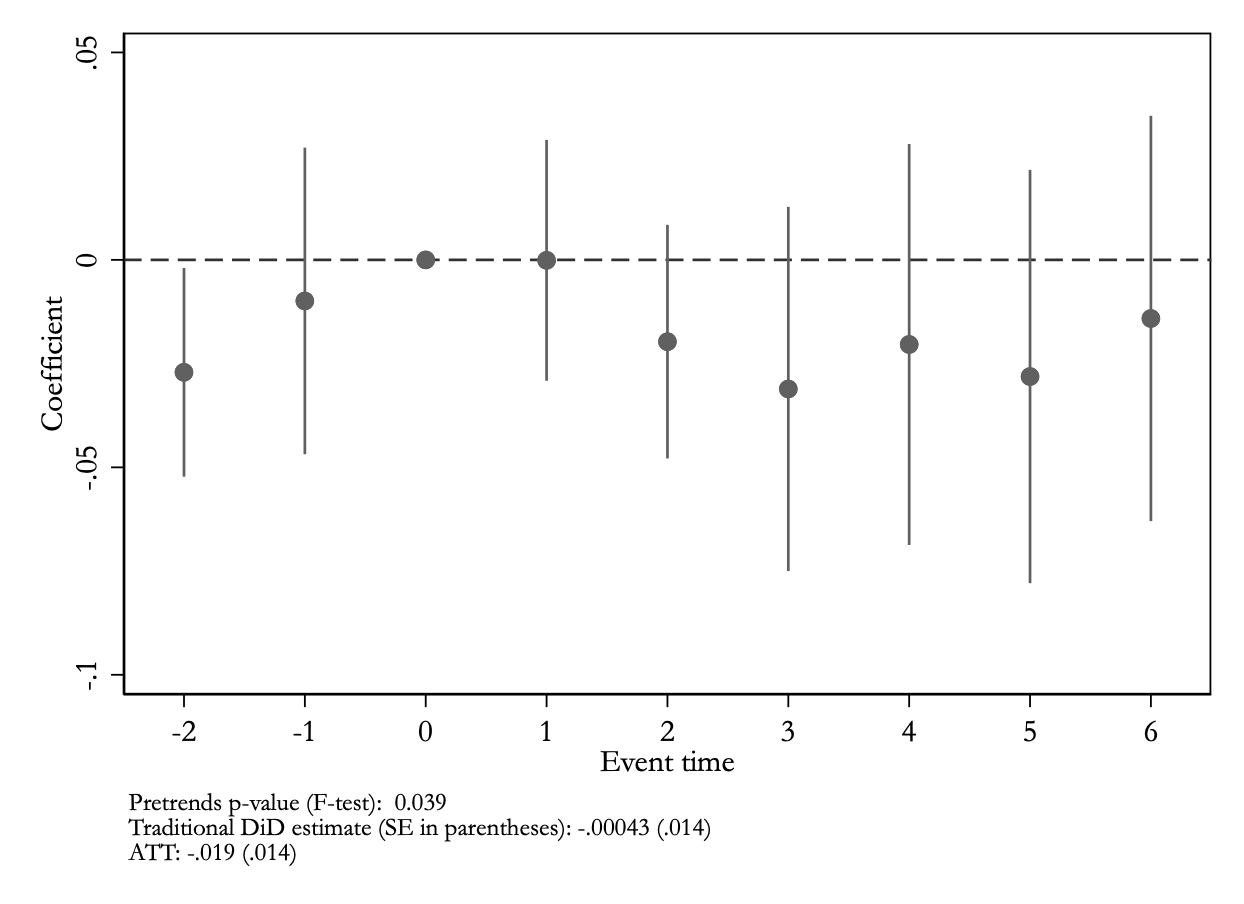
\includegraphics[width=7cm]{eventstudy/high_drug_use/reducedform_ab1986.png} }}%
  \qquad
  \subfloat[\centering Using juvenile arrests]{{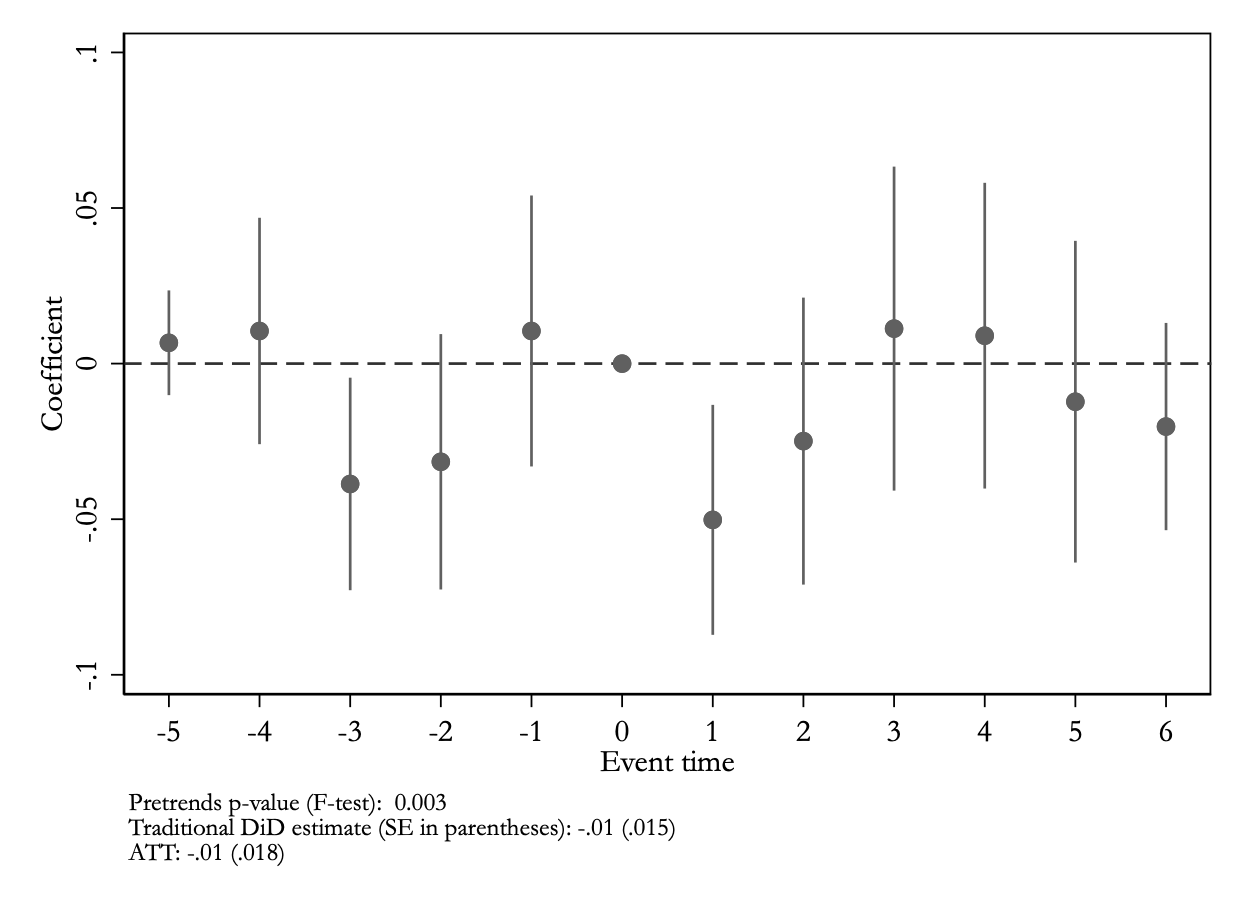
\includegraphics[width=7cm]{eventstudy/high_drug_use/reducedform_jb2010.png} }}%
  \label{fig:rf_jb_es_2010}%
\end{figure}

\begin{footnotesize}
  \noindent Note: These figures report coefficients from the estimation of equation 1 evaluating the impact of the Fair Sentencing Act of 2010 on college enrollment rates using CPS-UCR merged data from 2005-2015. Figure A defines high-intensity states using Black adult arrests, while Figure B defines high-intensity states using Black juvenile arrests. Event time $0 \coloneqq 2010$. The coefficients represent the change in outcomes for high black adult drug arrest states relative to non-high-drug arrest states, where high-drug arrest states are defined to be those above the 75th percentile in 2008. The sample is defined as black males aged 18-24 in 2010 who were not incarcerated at the time of the survey. Control variables include population and unemployment rates at the state-year level. 
\end{footnotesize}

\clearpage
